\documentclass[hyperref={pdfpagelabels=false}]{beamer}

\usepackage[absolute, overlay]{textpos}
\usepackage{graphicx}
\usepackage{booktabs}
\usepackage{multirow}
\usepackage{subcaption}
\usepackage[round]{natbib}
\usepackage[titlenumbered, ruled]{algorithm2e}

\usetheme[progressbar=frametitle]{metropolis}           % Use metropolis theme
\setsansfont[Scale=0.8, BoldFont={FiraSans-Bold.ttf}]{FiraSans-Light.ttf}
\setmonofont[Scale=0.8, BoldFont={FiraMono-Bold.ttf}]{FiraMono-Regular.ttf}
\DeclareGraphicsExtensions{.pdf,.png,.jpeg,.jpg}
\graphicspath{{../img/sample/}{../img/moches/}{../img/original/}{../img/}}

\title{Contributions aux communications multi-vues\\pour l'apprentissage collaboratif}
\date{10 Décembre 2018}
\author{Denis Maurel}

\begin{document}

    \titlegraphic{%
        \begin{columns}
            \begin{column}{0.4\textwidth}
                \flushleft{
                    \resizebox{1.0\textwidth}{!}{
                        \begin{tabular}{r@{\ }ll}
                            & Mme. Raja {\sc Chiky} & Directrice de th\`{e}se\\
                            & M. Antoine {\sc Cornu\'{e}jols} & Examinateur \\
                            & Mme. Pascale {\sc Kuntz} & Rapportrice \\
                            & M. Sylvain {\sc Lefebvre} & Encadrant \\
                            & M. Christophe {\sc Marsala} & Examinateur \\
                            & M. Marcilio {\sc de Souto} & Examinateur \\
                            & M. J\'{e}r\'{e}mie {\sc Sublime} & Encadrant \\
                            & Mme. Rosanna {\sc Verde} & Rapportrice \\
                        \end{tabular}
                    }
                }
            \end{column}
            \begin{column}{0.55\textwidth}
                \begin{figure}[b]
                    \hfill
                    \begin{subfigure}[c]{0.4\textwidth}
                        
\includegraphics[width=\textwidth]{isep}
                    \end{subfigure}
                    \qquad
                    \begin{subfigure}[c]{0.4\textwidth}
                        
\includegraphics[width=\textwidth]{logo}
                    \end{subfigure}
                \end{figure}
            \end{column}
        \end{columns}
    }

    \makeatletter
    \setbeamertemplate{title page}{%
        \begin{minipage}[b][\paperheight]{\textwidth}
            \vfill%
            \ifx\inserttitle\@empty\else\usebeamertemplate*{title}\fi
            \ifx\insertsubtitle\@empty\else\usebeamertemplate*{subtitle}\fi
            \usebeamertemplate*{title separator}
            \ifx\beamer@shortauthor\@empty\else\usebeamertemplate*{author}\fi
            \ifx\insertdate\@empty\else\usebeamertemplate*{date}\fi
            \ifx\insertinstitute\@empty\else\usebeamertemplate*{institute}\fi
            \vfill
            \ifx\inserttitlegraphic\@empty\else\inserttitlegraphic\fi
            \vspace*{1cm}
        \end{minipage}
    }
    \makeatother


    \maketitle

    \begin{frame}{Plan}
        \setbeamertemplate{section in toc}{%
            {\inserttocsectionnumber.}~\inserttocsection
        }
        \tableofcontents[hideallsubsections]
	\end{frame}

    \section{Introduction}
    \begin{frame}{Clustering collaboratif: définition}
        Le \textbf{clustering collaboratif} est un domaine récent
        ([Pedrycz2002]) désignant l'ensemble des méthodes permettant à
        \textbf{plusieurs algorithmes de clustering} opérant sur des
        \textbf{sources de données différentes et indépendantes} de collaborer
        pour \textbf{améliorer localement} leurs résultats.

        \begin{figure}[b]
            \centering
            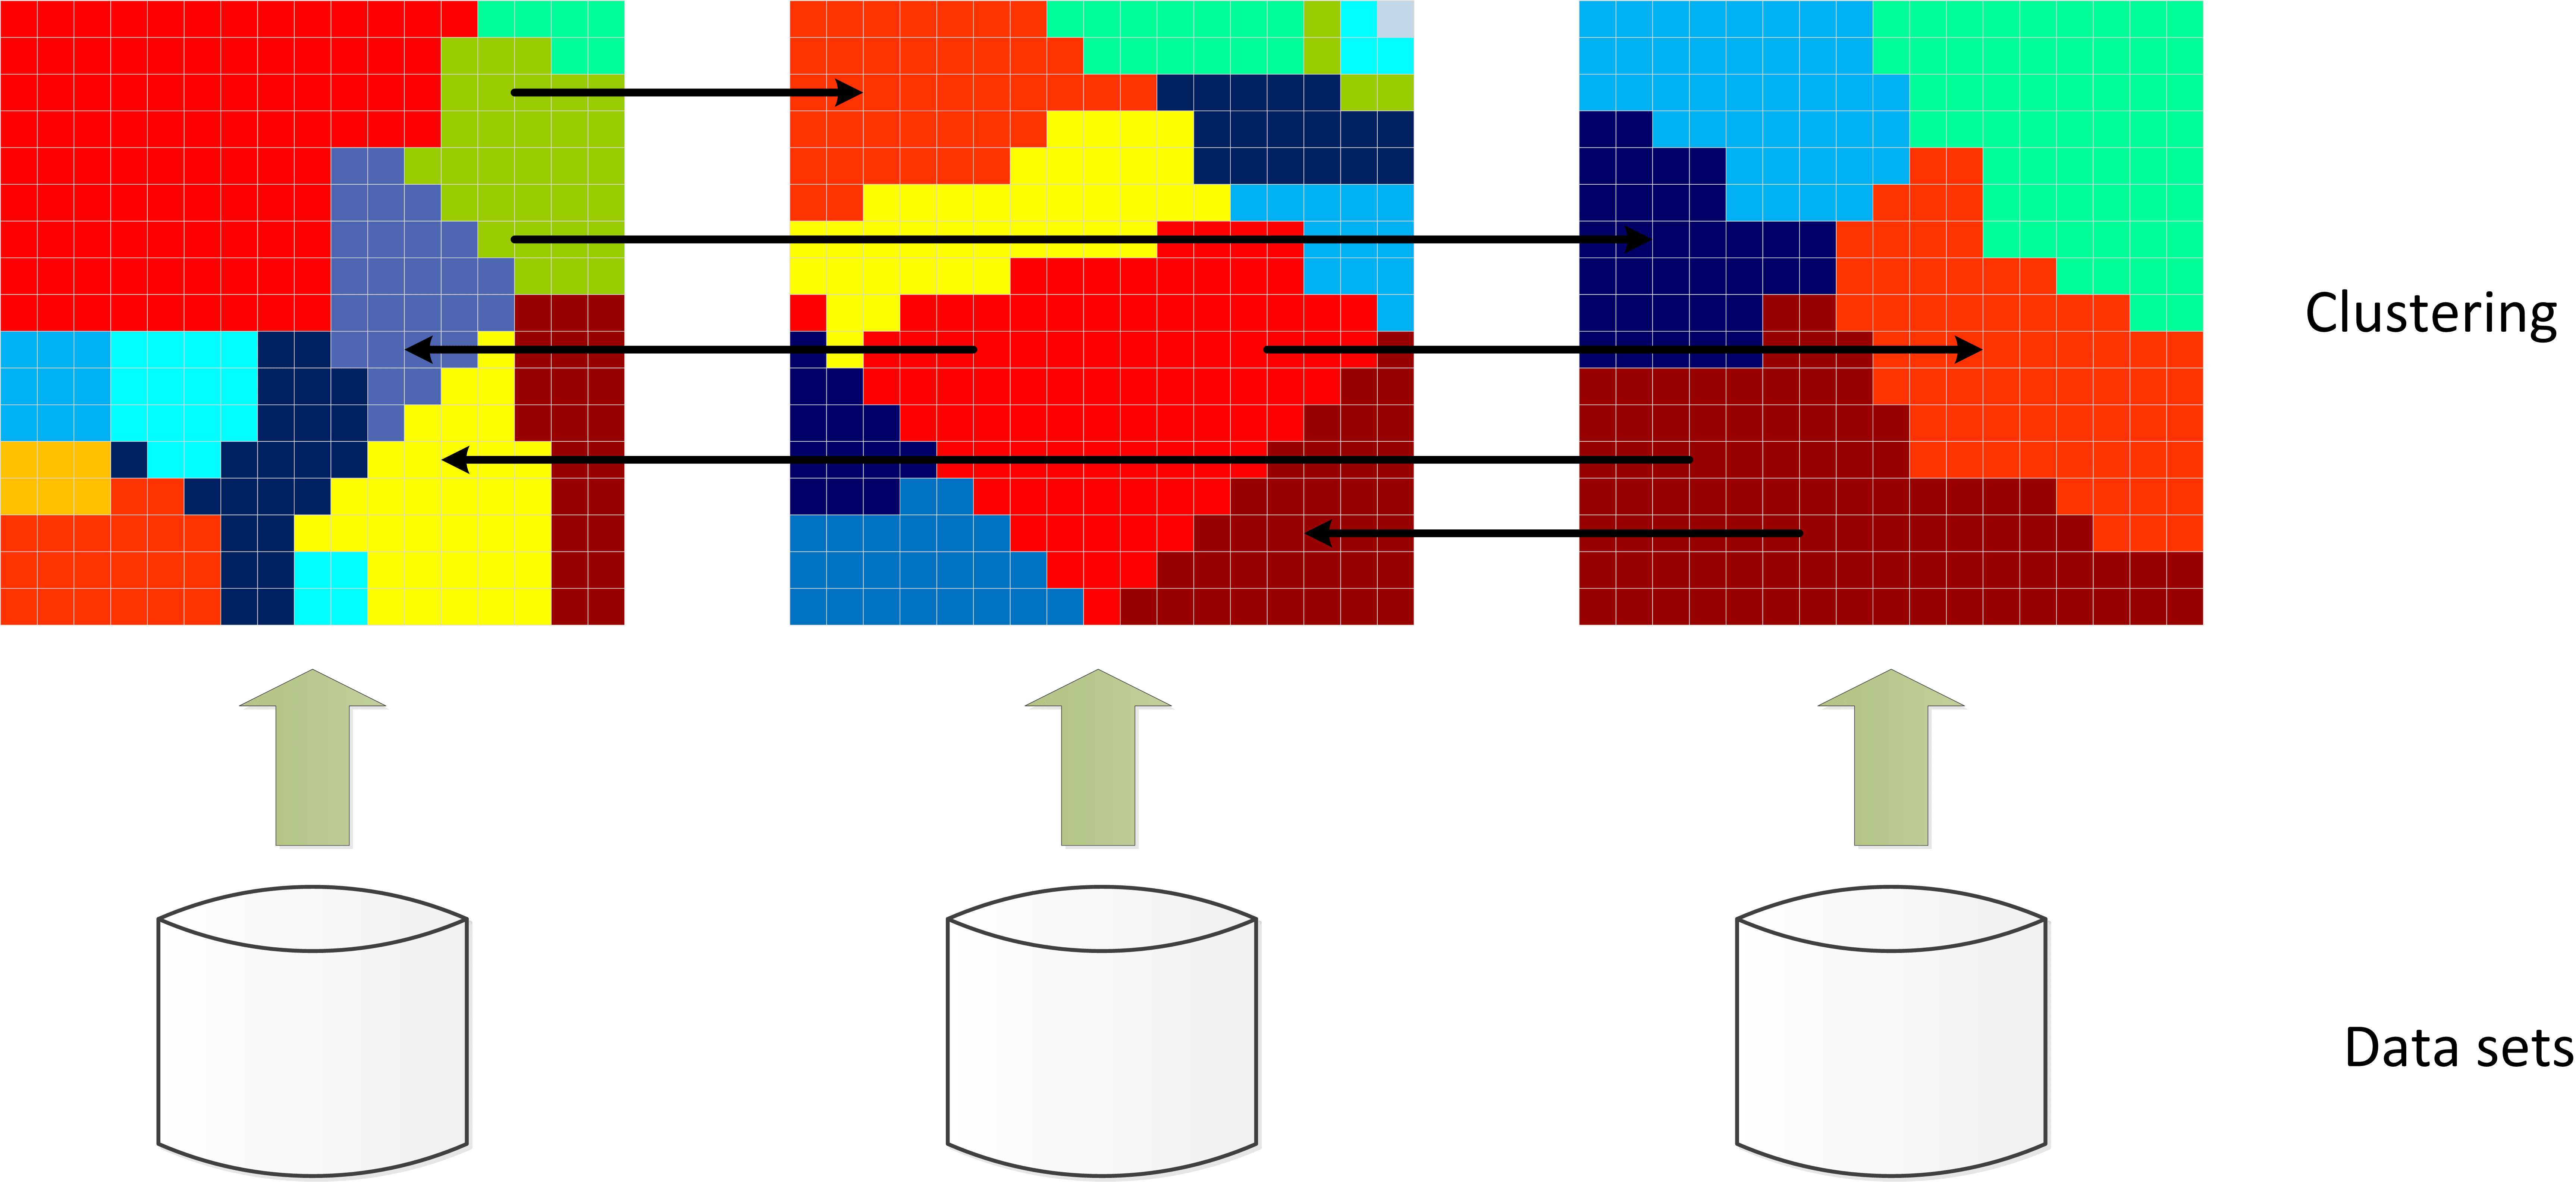
\includegraphics[scale=0.02]{hcc-min}
            \caption{Illustration du principe de clustering collaboratif 
            horizontal}
        \end{figure}
    \end{frame}

    \begin{frame}{Clustering collaboratif: définition}
        \begin{itemize}
            \item<+-> $N$ bases de données $\rightarrow$ \textbf{\textit{N} 
                vues}.
            \item<+-> Description du \textbf{même ensemble d'individus} pour 
                permettre l'analyse des \textbf{correspondances}:
            \item<+-> \textbf{\textit{N} algorithmes de clustering} 
                (potentiellement différents)
                $\rightarrow$ 1 par vue.
                \begin{itemize}
                    \item SOM [Grozavu2010], Fuzzy C-Means [Pedrycz2004], GTM
                        [Ghassany2012]
                \end{itemize}
            \item<+-> 2 phases: phase \textbf{locale} et phase 
                \textbf{collaborative} [Pedrycz2002]
        \end{itemize}

        \onslide<+->{
            Avantages:
            \begin{itemize}
                \item Prise en compte \textbf{d'informations externes} dans les 
                    résultats locaux
                \item \textbf{Adaptation des méthodes de clustering} suivant la 
                    source de données
                \item Répartition de la \textbf{charge de calcul} sur l'ensemble des 
                    vues.
                \item \textbf{Sécurisation} des données transférées
            \end{itemize}
        }
    \end{frame}

    \begin{frame}{Clustering collaboratif: processus}
        \begin{figure}[b]
            \centering
            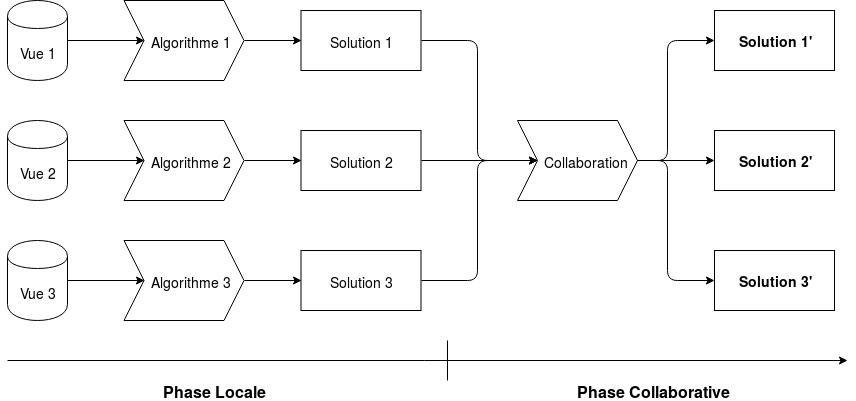
\includegraphics[scale=.35]{cc_resume}
            \caption{Processus de clustering collaboratif}
        \end{figure}
    \end{frame}

    %\begin{frame}{Clustering collaboratif: théorie}
        %Définition d'un critère $Q^i$ à optimiser pour chaque vue $V_i$:
        %\begin{align*}
            %$Q^i &= \alpha_i Q^i_{local}(V_i) + Q^i_{collab}(V_i, V_{j\neq i})\\
            %&= \alpha_i Q^i_{local}(V_i) + \sum_{j\neq i} \beta^i_j C_j^i(V_i, V_j)$
        %\end{align*}
        %Avec:
        %\begin{itemize}
            %\item $\alpha_i$ et $\beta_j^i$ les coeffcients de pondération.
            %\item $Q^i_{local}$ et $Q^i_{collab}$ respectivement les 
                %contributions de la vue locale et des vues externes.
            %\item $C_j^i$ la contribution de la vue externe $V_j$, détermine le 
                %degrès de similarité entre $V_i$ et $V_j$.
        %\end{itemize}
    %\end{frame}

    \begin{frame}{Clustering collaboratif: théorie}
        Définition du critère collaboratif:
        \begin{align}
            Q^i &= \alpha_i Q^i_{local}(V_i) + Q^i_{collab}(V_i, V_{j\neq i})\\
            &= \alpha_i Q^i_{local}(V_i) + \sum_{j\neq i} \beta^i_j C_j^i(V_i, 
            V_j)
        \end{align}
        \begin{itemize}
            \item $Q^i_{local}$ est généralement basé sur \textbf{le critère de 
                l'algorithme local} à optimiser.
            \item $Q^i_{collab}$ se base sur \textbf{l'échange d'information 
                entre vues}, typiquement les appartenances des individus aux 
                clusters respectifs de chaque vue.
            \item $C_j^i$ représente \textbf{la dissimilarité} entre les vues i 
                et j.
            \item $\alpha_i$ et $\beta_j^i$ sont définis \textbf{à la main}.  
                L'approximation $\forall j, \beta_j^i = \alpha_i^2$ est parfois 
                utilisée car donnant de bons résultats en pratique [Grozavu2011].
        \end{itemize}
    \end{frame}

    \begin{frame}{Problématique}
            \begin{center}
                \fontsize{14pt}{15pt}
                \textbf{Comment améliorer les communications opérées durant un 
                apprentissage collaboratif ?}
            \end{center}
    \end{frame}

    \begin{frame}{Contributions}
        Réponse à la problématique suivant 3 axes:
        \begin{enumerate}
            \item<+(1)-> Rendre le clustering collaboratif \textbf{incrémental}.
                \begin{itemize}
                    \item (article) ICONIP 2017
                    \item (article) EGC 2018
                \end{itemize}
            \item<+(1)-> \textbf{Détection automatique} des meilleures 
                collaboration inter-vues.
                \begin{itemize}
                    \item (article) IJCNN 2018
                \end{itemize}
            \item<+(1)-> Ouverture du paradigme collaboratif au problème de la 
                \textbf{reconstruction}.
                \begin{itemize}
                    \item (journal, en cours de soumission) KAIS
                \end{itemize}
        \end{enumerate}
    \end{frame}

    \section{Clustering collaboratif incrémental}
        \begin{frame}{Contexte}
            \textit{Objectif du clustering collaboratif}: définir un ensemble de 
            clusters suivant \textbf{la distribution} des données fournies en 
            entrée.

            \textbf{Problème}: il arrive que cette distribution \textbf{évolue 
            au cours du temps}

            \textbf{Exemple}: évolution du régime alimentaire d'un individu ou 
            de la répartition des salaires à l'échelle d'une population.

            \begin{figure}[b]
                \centering
                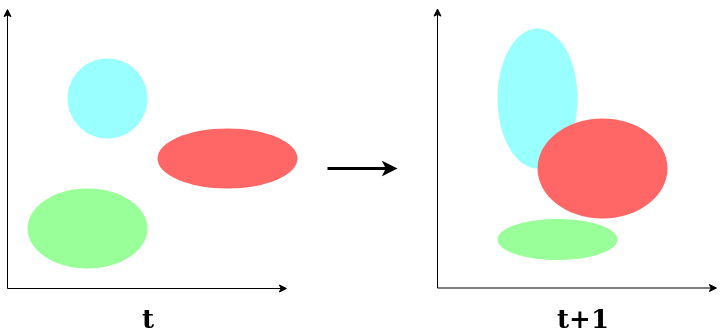
\includegraphics[scale=.2]{changedistrib}
            \end{figure}

            Utilisation du clustering \textbf{incrémental}: les clusters sont 
            appris au cours du temps afin de \textbf{s'adapter} aux éventuels 
            changements de distribution. On utilise les $N_{batch}$ derniers 
            individus comme échantillon d'apprentissage.

        \end{frame}

        \begin{frame}{Clustering collaboratif incrémental}
            Définition d'une méthode de clustering incrémental:
            \begin{itemize}
                \item<2-> Choix de la \textbf{méthode de clustering}
                \item<3-> \textbf{Adaptation de la méthode de clustering} pour 
                    de l'apprentissage incrémental
                \item<4-> \textbf{Adaptation du clustering collaboratif} au 
                    modèle de clustering obtenu
            \end{itemize}
        \end{frame}

        \begin{frame}{Cartes Auto-Adaptatrices (SOM)}
            Dans notre cas, utilisation des \textbf{cartes auto-adaptatrices de
            Kohonen} (ou Self-Organizing Maps (SOM) en anglais) [Kohonen1982]
            comme méthode de clustering.
            \begin{itemize}
                \item Méthode à base de \textbf{prototypes} utilisée pour le
                    clustering collaboratif [Grozavu2010].
                \item Permet la \textbf{visualisation} de données en hautes 
                    dimensions
                \item Notion de \textbf{voisinage}: utilisation d'une 
                    \textbf{fonction de température}.
            \end{itemize}

            \begin{figure}[b]
                \centering
                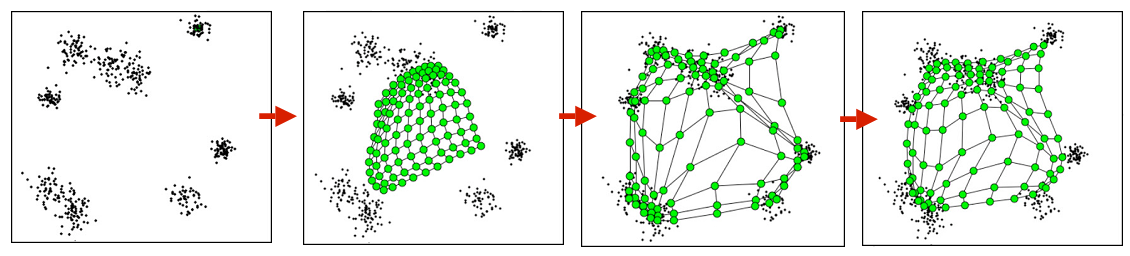
\includegraphics[scale=.43]{SOM2}
                \caption{Exemple de SOM}
            \end{figure}
        \end{frame}

        \begin{frame}{Cartes Auto-Adaptatrices (SOM)}
            \begin{center}
                
            \end{center}
            
            \begin{equation*}
                \text{Fonction de voisinage:} \qquad K_{i,j} = 
                \exp\left(-\frac{d^2_1(i,j)}{\lambda(t)}\right)
            \end{equation*}

            \begin{equation*}
                \text{Fonction de température:} \qquad
                \lambda(t) = 
                \lambda_{min}\left(\frac{\lambda_{max}}{\lambda_{min}}\right)^{\frac{1}{t}}
            \end{equation*}

            \begin{figure}[b]
                \centering
                \begin{subfigure}[b]{0.45\textwidth}
                    \centering
                    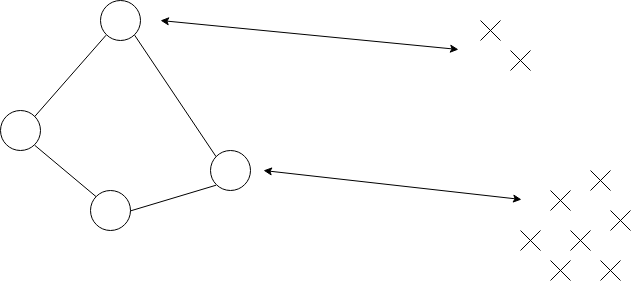
\includegraphics[scale=.20]{somhot}
                    \caption{Température élevée}
                \end{subfigure}
                \begin{subfigure}[b]{0.45\textwidth}
                    \centering
                    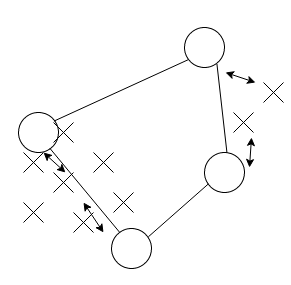
\includegraphics[scale=.25]{somcold}
                    \caption{Température faible}
                \end{subfigure}
            \end{figure}
        \end{frame}

        \begin{frame}{SOM incrémentale}
            %\begin{itemize}
                %\item \textbf{$\mathbf{1^{ère}}$ contrainte}: des individus 
                    %correspondants doivent appartenir à des \textbf{prototypes 
                    %correspondants} ou à leurs voisinnages proches.
                %\item \textbf{$\mathbf{2^{ème}}$ contrainte}: \textbf{même 
                    %topologie des cartes} pour toutes les vues pour les rendre 
                    %comparables.
            %\end{itemize}

            Les solutions existantes pour les SOM incrémentales se basent toutes 
            sur l'ajout de prototypes ([Paplinski2012] et [Deng2000]).\\~\\
            \onslide<2->{\textbf{Problème 1}: Est-il possible de trouver une 
            solution \textbf{conservant la topologie de la carte} ?\\}
            \onslide<3->{\textbf{Problème 2}: $\lambda$ est \textbf{dépendante du 
            temps}, ce qui pose problème avec le clustering incrémental.\\~\\}

            %$\rightarrow$ \textbf{Non applicable au clustering collaboratif} du 
            %fait de la seconde contrainte.
            \onslide<4->{
                $\rightarrow$ rendre la fonction dépendante des 
                \textbf{individus}
                \begin{equation*}
                    \lambda(t) = 
                    \lambda_{min}\left(\frac{\lambda_{max}}{\lambda_{min}}\right)^{\frac{1}{t}}
                    \quad\rightarrow\quad
                    \widetilde{\lambda}(B, W) = 
                    \frac{1}{N_{batch}}\sum_{i=1}^{N_{batch}}\|x_i - 
                    \chi(x_i)\|_2
                \end{equation*}
                \begin{equation*}
                    K_{i,j}\left(\lambda(t)\right) \rightarrow 
                    K_{i,j}\left(\widetilde{  \lambda}(B,W)\right) \rightarrow 
                    \widetilde{K}_{i,j}
                \end{equation*}
                \vspace{.1cm}
            }
        \end{frame}

        %\begin{frame}{SOM incrémentale et clustering collaboratif}
            %L'application des SOM au clustering collaboratif se fait en 
            %définissant les termes précemment définis:

            %\begin{equation*}
            %{Q}^m_{local} = 
            %\alpha_m\sum_{i=1}^{N}\sum_{j=1}^{|W|}{K}^m_{j, 
            %\chi(x_i)}\|x_i^m - \omega_j^m\|^2
            %\end{equation*}

            %\begin{equation*}
            %{Q}^m_{collab} = \sum_{m'=1, m'\neq 
            %m}^{P}\beta_m^{m'}\sum_{i=1}^{N}\sum_{j=1}^{|W|}({K}^m_{j, 
            %\chi(x_i)} - {K}^{m'}_{j, \chi(x_i)})^2  \|x_i^m - \omega_j^m\|^2
            %\end{equation*}

            %\begin{itemize}
                %\item $W$ $\rightarrow$ la carte de prototypes
                %\item $\chi(x_i)$ $\rightarrow$ la fonction retournant le 
                    %prototype le plus proche de $x_i$.
                %\item $x_i^k$ $\rightarrow$ l'individu $i$ dans la vue $m$
                %\item $\omega_j^m$ $\rightarrow$ le prototype $j$ de la SOM de 
                    %la vue m.
            %\end{itemize}
        %\end{frame}
    

        \begin{frame}{SOM incrémentale et clustering collaboratif}
            \begin{itemize}
                \item<2-> \textbf{$\mathbf{1^{ère}}$ contrainte}: des individus 
                    correspondants doivent appartenir à des \textbf{prototypes 
                    correspondants} ou à leurs voisinnages proches.
                \item<3-> \textbf{$\mathbf{2^{ème}}$ contrainte}: \textbf{même 
                    topologie des cartes} pour toutes les vues pour les rendre 
                    comparables.
            \end{itemize}

            \onslide<4->{
                \begin{columns}
                    \begin{column}{0.6\textwidth}
                        \begin{align*}
                            & Q_{local}^m(K_{i,j}) \quad / \quad Q_{collab}^m ( 
                            K^m_{i,j} - K^{m'}_{i,j}) \\
                            \Rightarrow\quad & Q_{local}^m(\widetilde{K}_{i,j}) 
                            \quad / \quad Q_{collab}^m ( \widetilde{K}^m_{i,j} - 
                            \widetilde{K}^{m'}_{i,j})\\
                            \Rightarrow\quad & \widetilde{Q}_{local}^m \quad / 
                            \quad \widetilde{Q}_{collab}^m
                        \end{align*}
                    \end{column}
                    \begin{column}{0.4\textwidth}
                        \begin{equation*}
                            \widetilde{K}_{i,j} = 
                            \exp\left(-\frac{d^2_1(i,j)}{\widetilde{\lambda}(B, W)}\right)
                        \end{equation*}
                    \end{column}
                \end{columns}
                Le nouveau critère dépendant uniquement des $N_{batch}$ derniers 
                individus apparus, il est possible d'effectuer un 
                \textbf{apprentissage collaboratif incrémental} sur l'ensemble des 
                vues.
            }

            %Les règles de mise à jour sont obtenus par \textbf{descente de 
            %gradient} appliquée sur ce critère.
        \end{frame}

        %\begin{frame}{Expérimentations}
            %\begin{itemize}
                %\item Analyse de l'impact du clustering collaboratif sur
                    %l'apprentissage incrémental.
                %\item Application directe de la phase collaborative pour le
                    %clustering collaboratif pour pouvoir comparer les
                    %résultats aux version locales.
                %\item Variation de la taille du batch pour étudier l'impact
                    %sur l'apprentissage.
            %\end{itemize}
        %\end{frame}
        
        \begin{frame}{Expérimentations}
            Test de notre méthode sur 4 jeux de données différents
            \begin{itemize}
                \item Spambase
                \item Waveform
                \item Wisconsin Breast Cancer Diagnosis (WDBC)
                \item Isolet
            \end{itemize}

            \textbf{Pureté d'un prototype}: classe majoritaire parmi les
            individus associés à ce prototype.\\
            \textbf{Pureté d'une SOM}: pureté moyenne de ses prototypes.\\
            \textbf{Erreur moyenne de quantification}: distance moyenne
            entre un prototype et les individus qui y sont associés.

            \begin{equation*}
                qe = \frac{1}{N_{batch}}\sum_{i=1}^{N_{batch}}\|x_i -
                \chi(x_i)\|^2
            \end{equation*}
        \end{frame}

        \begin{frame}{Expérimentations: résultats}
            \begin{table}[!h]
                \caption{Erreur de quantification moyenne pour chaque base
                de donnée.}
                \begin{center}
                    \begin{tabular}{cccc}
                              & SOM incrémentales & 
                              \begin{tabular}[c]{@{}c@{}}clustering 
                              collaboratif\\ incrémental\end{tabular} & Gain            
                              \\ \hline
                    Spam Base & 0.223             & 0.203                                                                         
                    & \textbf{+ 8.9\%}  \\ \hline
                    Waveform  & 0.197             & 0.24                                                                          
                    & \textbf{- 21.8\%} \\ \hline

                    WDBC      & 0.183             & 0.18                                                                          
                    & \textbf{+ 1,6\%} \\ \hline
                    Isolet    & 2.61              & 1.34                                                                          
                    & \textbf{+ 48,7\%}
                    \end{tabular}
                \end{center}
            \end{table}
            \begin{itemize}
                \item \textbf{Score en quantification à long termes globalement 
                    comparables}: le clustering collaboratif n'endommage pas les 
                    résultats locaux.
                \item Le clustering collaboratif est sensible \textbf{à la 
                    présence de vues bruitées}.
            \end{itemize}
        \end{frame}

        \begin{frame}{Expérimentations: résultats sur Isolet}
            \begin{figure}[!h]
                \centering
                \caption{Évolution des puretés pour Isolet. Chaque itération correspond à l'arrivée d'un nouveau batch.}
                \begin{subfigure}[b]{0.3\textwidth}
                    \centering
                    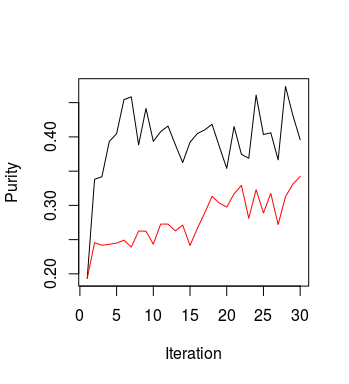
\includegraphics[width=0.7\textwidth, trim= 0cm 0.5cm 1cm 2cm, clip]{img/11.png}
                    \caption{$N_{batch}=10$, View 1}
                \end{subfigure}
                \begin{subfigure}[b]{0.3\textwidth}
                    \centering
                    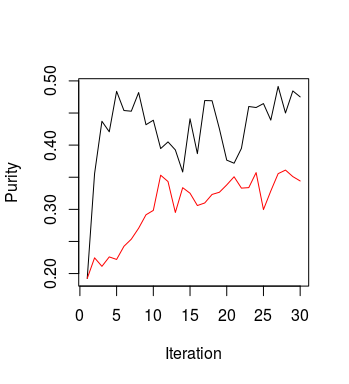
\includegraphics[width=0.7\textwidth, trim= 0cm 0.5cm 1cm 1.73cm, clip]{img/22.png}
                    \caption{$N_{batch}=10$, View 2}
                \end{subfigure}
                \begin{subfigure}[b]{0.3\textwidth}
                    \centering
                    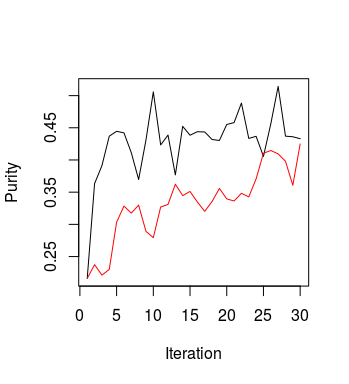
\includegraphics[width=0.7\textwidth, trim= 0cm 0.5cm 1cm 2cm, clip]{img/33.png}
                    \caption{$N_{batch}=10$, View 3}
                \end{subfigure}\\
                %\begin{subfigure}[b]{0.3\textwidth}
                    %\centering
                    %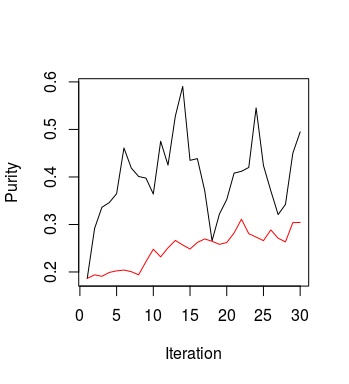
\includegraphics[width=0.7\textwidth, trim= 0cm 0.5cm 1cm 1.9cm, clip]{img/p1.png}
                    %\caption{$N_{batch}=3$, View 1}
                %\end{subfigure}
                %\begin{subfigure}[b]{0.3\textwidth}
                    %\centering
                    %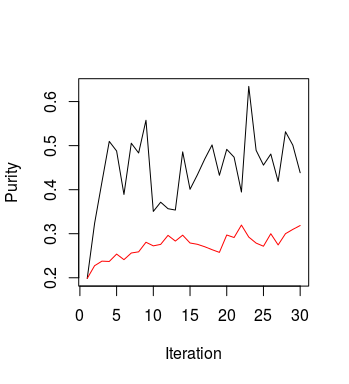
\includegraphics[width=0.7\textwidth, trim= 0cm 0.5cm 1cm 2cm, clip]{img/p2.png}
                    %\caption{$N_{batch}=3$, View 2}
                %\end{subfigure}
                %\begin{subfigure}[b]{0.3\textwidth}
                    %\centering
                    %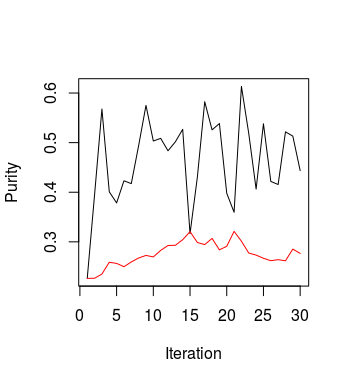
\includegraphics[width=0.7\textwidth, trim= 0cm 0.5cm 1cm 2cm, clip]{img/p3.png}
                    %\caption{$N_{batch}=3$, View 3}
                %\end{subfigure}
            \end{figure}
            \begin{center}
                {\color{red}SOM incrémentales} - \textbf{SOM incrémentales
                collaboratives}
            \end{center}
            \begin{itemize}
                \item Les SOM incrémentales collaboratives \textbf{apprennent 
                    plus vite que les SOM incrémentales seules}:                 
                    exploitation de l'information via le partage.
                \item Les SOM collaboratives sont globalement \textbf{plus 
                    instables} que les SOM incrémentales.
            \end{itemize}
        \end{frame}

        \begin{frame}{Expérimentations: résultats}
            \begin{figure}[!h]
                \centering
                \begin{subfigure}[b]{0.3\textwidth}
                    \centering
                    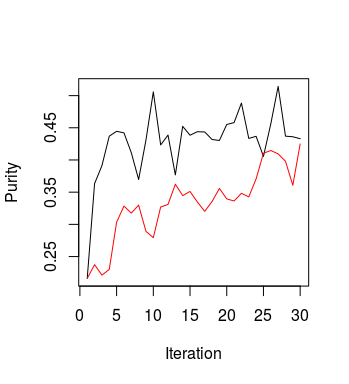
\includegraphics[width=0.7\textwidth, trim= 0cm 0.5cm 1cm 2cm, clip]{img/33.png}
                    \caption{$N_{batch}=10$, View 3}
                \end{subfigure}
                \begin{subfigure}[b]{0.3\textwidth}
                    \centering
                    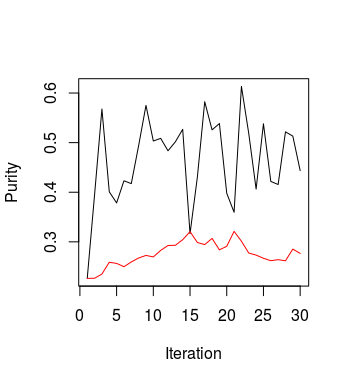
\includegraphics[width=0.7\textwidth, trim= 0cm 0.5cm 1cm 2cm, clip]{img/p3.png}
                    \caption{$N_{batch}=3$, View 3}
                \end{subfigure}
                \caption{Évolution des puretés pour Isolet: impact de la taille 
                du batch sur la stabilité de l'apprentissage.}
            \end{figure}
            \begin{itemize}
                \item La stabilité de l'apprentissage \textbf{augmente avec la 
                    taille du batch}: plus d'informations à exploiter.
            \end{itemize}
        \end{frame}

        \begin{frame}{Clustering collaboratif incrémental: résumé}
            Contributions
            \begin{itemize}
                \item Définition d'une \textbf{nouvelle méthode de cartes
                    auto-adaptatives incrémentales}
                \item Adaptation de la méthode précédente au \textbf{clustering
                    collaboratif}
                \item Analyse de l'impact de \textbf{la taille du batch sur la 
                    stabilité de l'apprentissage}.
            \end{itemize}

            \begin{center}
                \fontsize{14pt}{15pt}
                \onslide<2>{\textbf{Comment déterminer quelles sont les 
                    meilleures collaborations inter-vues ?}
                }
            \end{center}
        \end{frame}

    \section{Optimisation de paramètres pour le clustering collaboratif}

    \begin{frame}{Optimisation de paramètres pour le clustering collaboratif}
        Rappel du critère du clustering collaboratif:
        \begin{align*}
            Q^i &= \alpha_i Q^i_{local}(V_i) + Q^i_{collab}(V_i, 
            V_{j\neq i})\\
            &= \alpha_i Q^i_{local}(V_i) + \sum_{j\neq i} \beta^i_j 
            C_j^i(V_i, V_j)
        \end{align*}

        \textbf{Objectif}: Apprendre automatiquement les $\alpha$ et les
        $\beta$ en s'affranchissant de simplifications telles que $\beta =
        \alpha^2$.

        Nous proposons \textbf{une nouvelle méthode de pondération} permettant 
        d'apprendre automatiquement les poids fixant \textbf{les importances 
        relatives des différents scores}.\\
    \end{frame}

    \begin{frame}{Optimisation de paramètres: définition du problème}
        La définition des $\alpha$ et des $\beta$ passe par la résolution
        d'un problème sous contrainte. Les contraintes sont les suivantes :

        \begin{itemize}
            \item<2->{Affranchissement des $\alpha$: comme il s'agit de 
                pondérations relatives, on peut fixer $\alpha=1$.}
            \item<3-> $\beta^* =  
                \operatornamewithlimits{argmin}_{\beta}  \sum_{i \neq j}
        \beta_{i,j}  C _{i,j} $
            \item<4-> $\forall j \quad \prod_{i \neq j}^J \beta_{i,j} = 
                1$ (prise en compte des avis \textbf{divergents})
            \item<5-> $\forall (i,j) \quad \beta_{i,j} >0$
        \end{itemize}

        \onslide<6->{\textbf{Objectif:} mettre des poids plus élevés sur 
            les meilleurs accords, tout en gardant une certaine partie 
            des vues en désaccord pour faire évoluer l'information
        }
    \end{frame}

    \begin{frame}{Optimisation de paramètres: méthode de Karush-Kuhn-Tucker}
        Extension de la méthode du multiplateur de Lagrange aux contraintes 
        d'inégalités\\
        $\rightarrow$ \textbf{méthode de Karush-Kuhn-Tucker (KKT)} [Kuhn1951]. 

        \begin{equation*}
        L(\beta,\nu,\lambda)=\sum_{j=1}^J  \sum_{i \neq j}^J ( \beta_{i,j}  C_j^i
        - \nu_j  \ln  \beta_{i,j}  - \lambda_{i,j}   \beta_{i,j} ).
        \end{equation*}

        \begin{equation*}
            \frac{\partial L}{\partial \beta_{i,j}} = 0,
            \quad
            \frac{\partial L}{\partial \nu} = 0,
            \quad
            \frac{\partial L}{\partial \lambda} = 0
        \end{equation*}
    \end{frame}
    
    \begin{frame}{Optimisation de paramètres: résultats}
        Après résolution, on obtient:

        \vspace{0.6cm}

        \begin{equation*}
            \forall (i,j), \quad i\neq j \qquad \beta_{i,j} =  
            \frac{(\prod_{k\neq j} C_k^i)^{\frac 
            1 {J-1}}}{C_j^i}
        \end{equation*} 

        \vspace{1cm}
        L'importance d'une vue externe relativement à une vue locale est
        proportionnelle au rapport entre la moyenne géométrique de toutes les
        dissimilarités sur la dissimilarité entre les deux vues
        .\\
        \onslide<2->{$\rightarrow$ \textbf{plus 2 vues sont similaires, 
            plus elles collaboreront.}
        }
    \end{frame}

    %\begin{frame}
        %\begin{algorithm}[H]
            %\caption{Algorithme topologique de collaboration horizontale}
            %\textbf{Initialisation:} Initialiser toutes les cartes de
            %prototypes $W$ aléatoirement. \\
            %\textbf{Étape locale:} Initialisation des cartes\\
            %\ForAll{Vue} {
                %Minimiser la fonction objectif des cartes auto-adaptatrices
                %standards.
            %} 
            %\textbf{Étape collaborative:}\\
            %\ForAll{Vue} {
                %Pour $w$ fixé, mettre à jour $\beta$\\
                %$ \beta^{*} =  argmin_{\beta}Q(w,\alpha,\beta) $\\
                %Pour $\beta$ fixés, mettre à jour les prototypes de 
                %toutes les cartes:\\
                %$ w^{*} =  argmin_{w}Q(w,\alpha,\beta) $
            %}	 
        %\end{algorithm}
    %\end{frame}

    \begin{frame}{Expérimentations}
        Deux axes d'analyse:
        \begin{itemize}
            \item Analyse de \textbf{l'évolution du critère collaboratif} avec 
                et sans apprentissage automatique des poids (critère: différence 
                relative).
            \item Analyse des \textbf{valeurs prises par les} $\beta$ en fin 
                d'apprentissage. (critère: différences relatives entre les 
                poids).
        \end{itemize}

        \onslide<2->{Ce que l'on s'attend à trouver:
            \begin{itemize}
                \item Une \textbf{amélioration de la valeur du critère 
                    collaboratif} grâce à notre méthode
                \item \textbf{L'identification automatique des vues 
                    bruitées}, menant à des valeurs de $\beta$ proches de 0.
            \end{itemize}
        }

        \onslide<3->{À noter: pour chaque base de données, \textbf{une 
            vue entièrement composée de bruit} a été rajoutée pour 
            tester le second point.
        }
    \end{frame}

    \begin{frame}{Expérimentations: évolution du critère}
        \begin{figure}[!h]
            \centering
            \caption{Différences relatives du critère collaboratif avec et sans 
                optimisation des $\beta$ tout au long du processus 
                d'apprentissage.
            }
            %\begin{subfigure}[b]{0.3\textwidth}
                %\centering
                %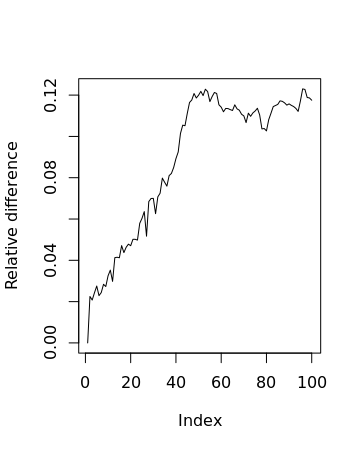
\includegraphics[width=0.8\textwidth]{wdbc_RD.png}
                %\caption{WDBC}
            %\end{subfigure}
            %\begin{subfigure}[b]{0.32\textwidth}
                %\centering
                %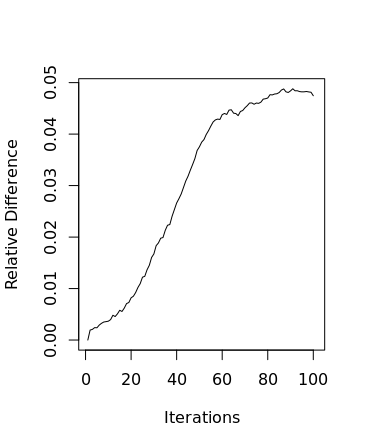
\includegraphics[width=1.0\textwidth]{waveform_RD2.png}
                %\caption{Waveform}
            %\end{subfigure}
            \begin{subfigure}[b]{0.32\textwidth}
                \centering
                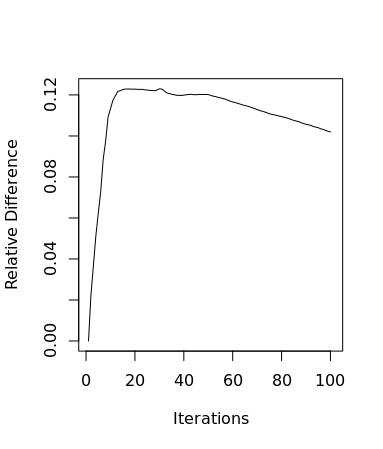
\includegraphics[width=0.8\textwidth]{vhr_RD}
                \caption{VHR Strasbourg}
            \end{subfigure}
            \begin{subfigure}[b]{0.32\textwidth}
                \centering
                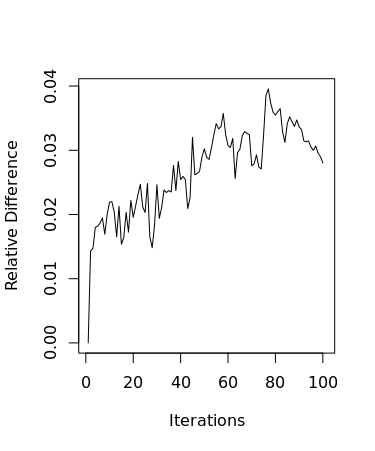
\includegraphics[width=0.8\textwidth]{isolet_RD2}
                \caption{Isolet}
            \end{subfigure}
            \begin{subfigure}[b]{0.32\textwidth}
                \centering
                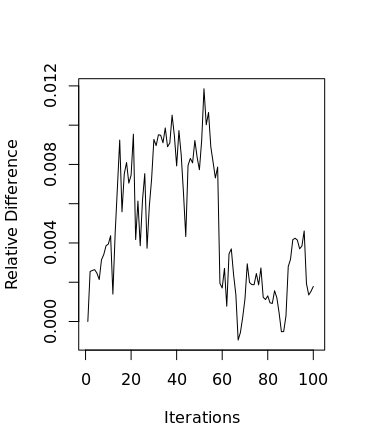
\includegraphics[width=0.8\textwidth]{spambase_RD3.png}
                \caption{Spambase}
            \end{subfigure}
        \end{figure}

        \begin{itemize}
            \item \textbf{Amélioration du critère} de manière significative dans 
                la majorité des cas
            \item Tous les jeux de données \textbf{ne sont pas traités de la 
                même manière} (dépend de la quantité et de la qualité de 
                l'informations à partager).
        \end{itemize}
    \end{frame}

    \begin{frame}{Expérimentations: identifications des vues bruitées}
        \begin{figure}[b]
            \centering
            \caption{Cartes de chaleur des matrices de $\beta$ pour chaque jeu 
                de données.\\$M(i,j)$ correspond à l'importance accordée à la 
                Vue j par la Vue i.\\Blanc = forte collaboration - noir = faible 
                collaboration -  diagonale représente $\beta=1$.
            }
            \begin{subfigure}[b]{0.32\textwidth}
                \centering
                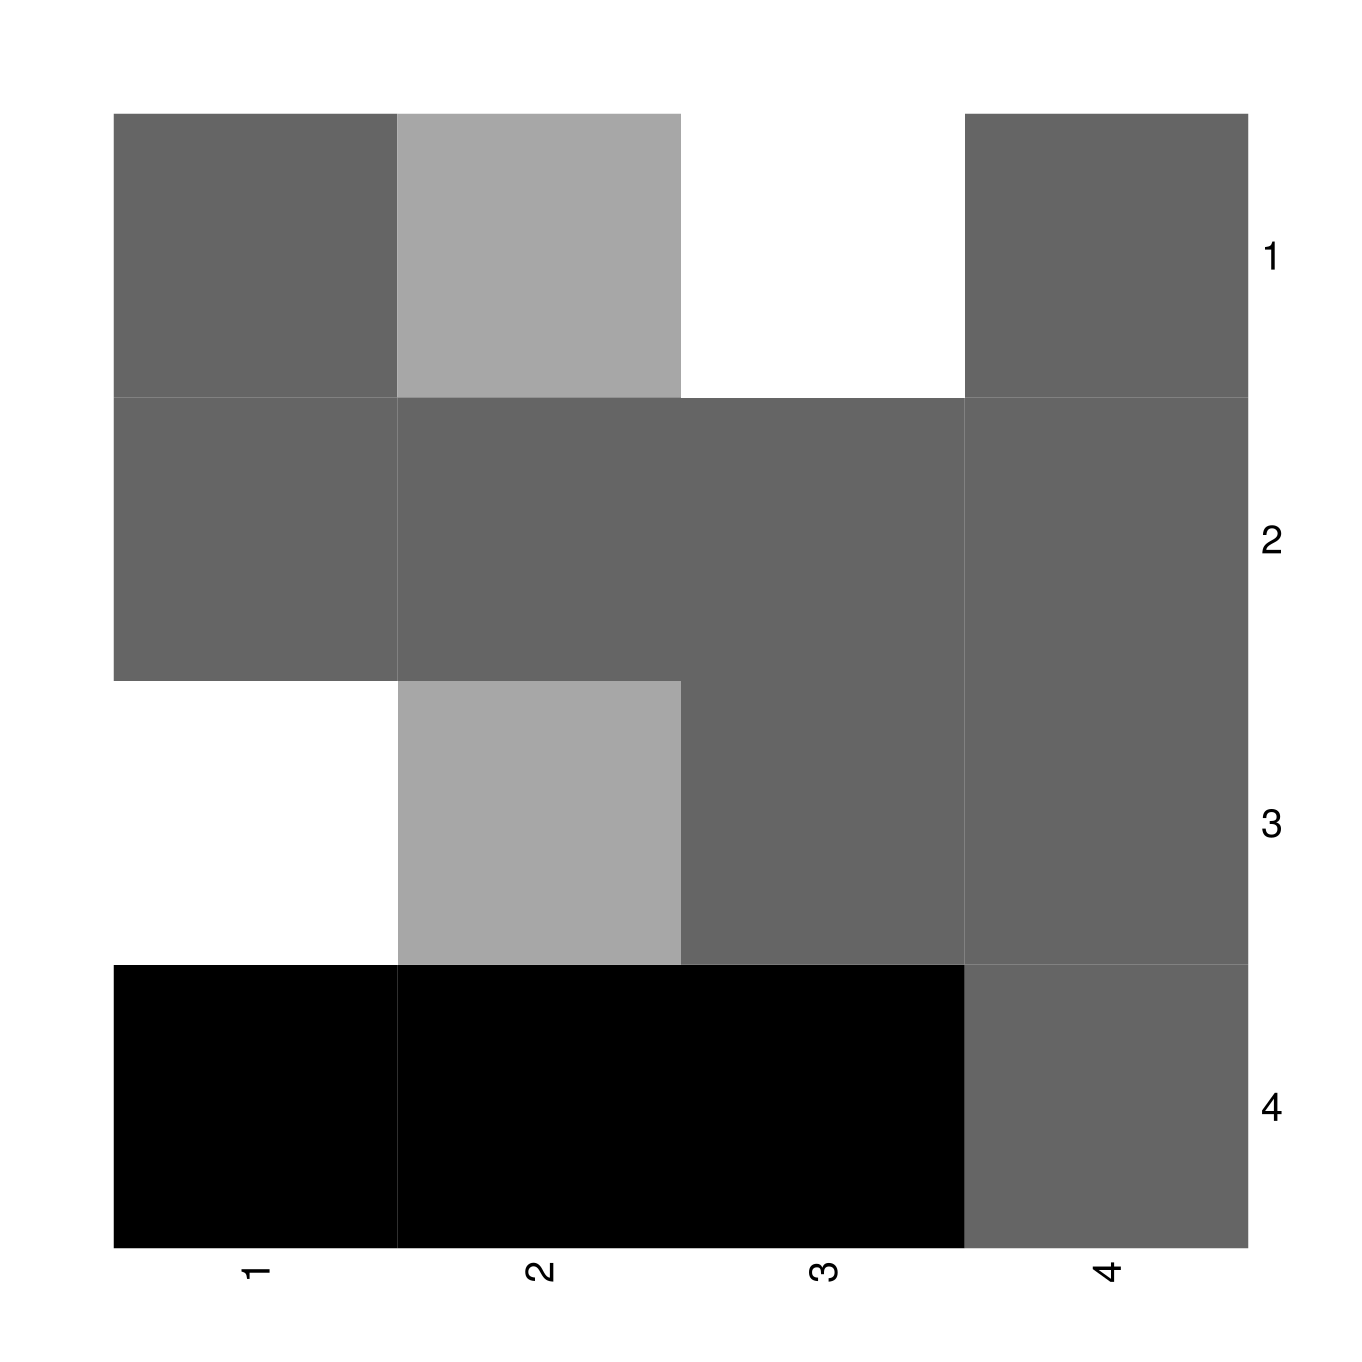
\includegraphics[width=0.8\textwidth]{wdbc_bw}
                \caption{WDBC}
            \end{subfigure}
            \begin{subfigure}[b]{0.32\textwidth}
                \centering
                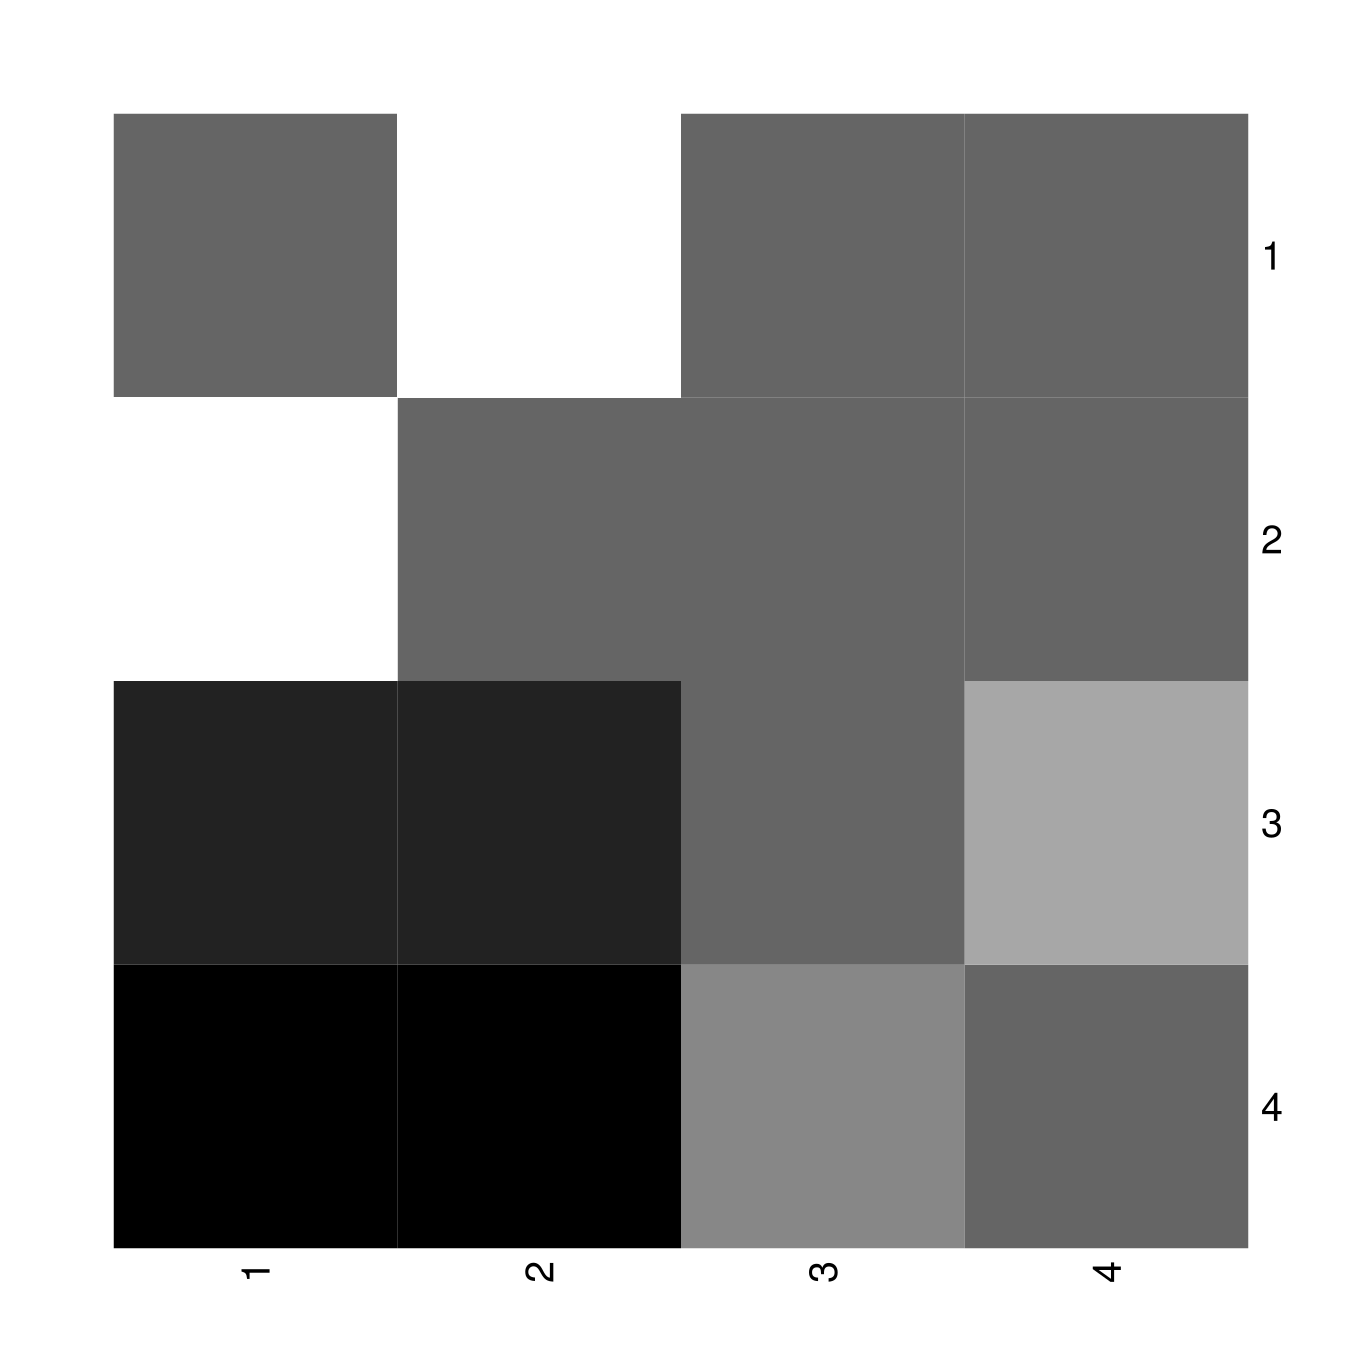
\includegraphics[width=0.8\textwidth]{waveform_bw}
                \caption{Waveform}
            \end{subfigure}
            \begin{subfigure}[b]{0.32\textwidth}
                \centering
                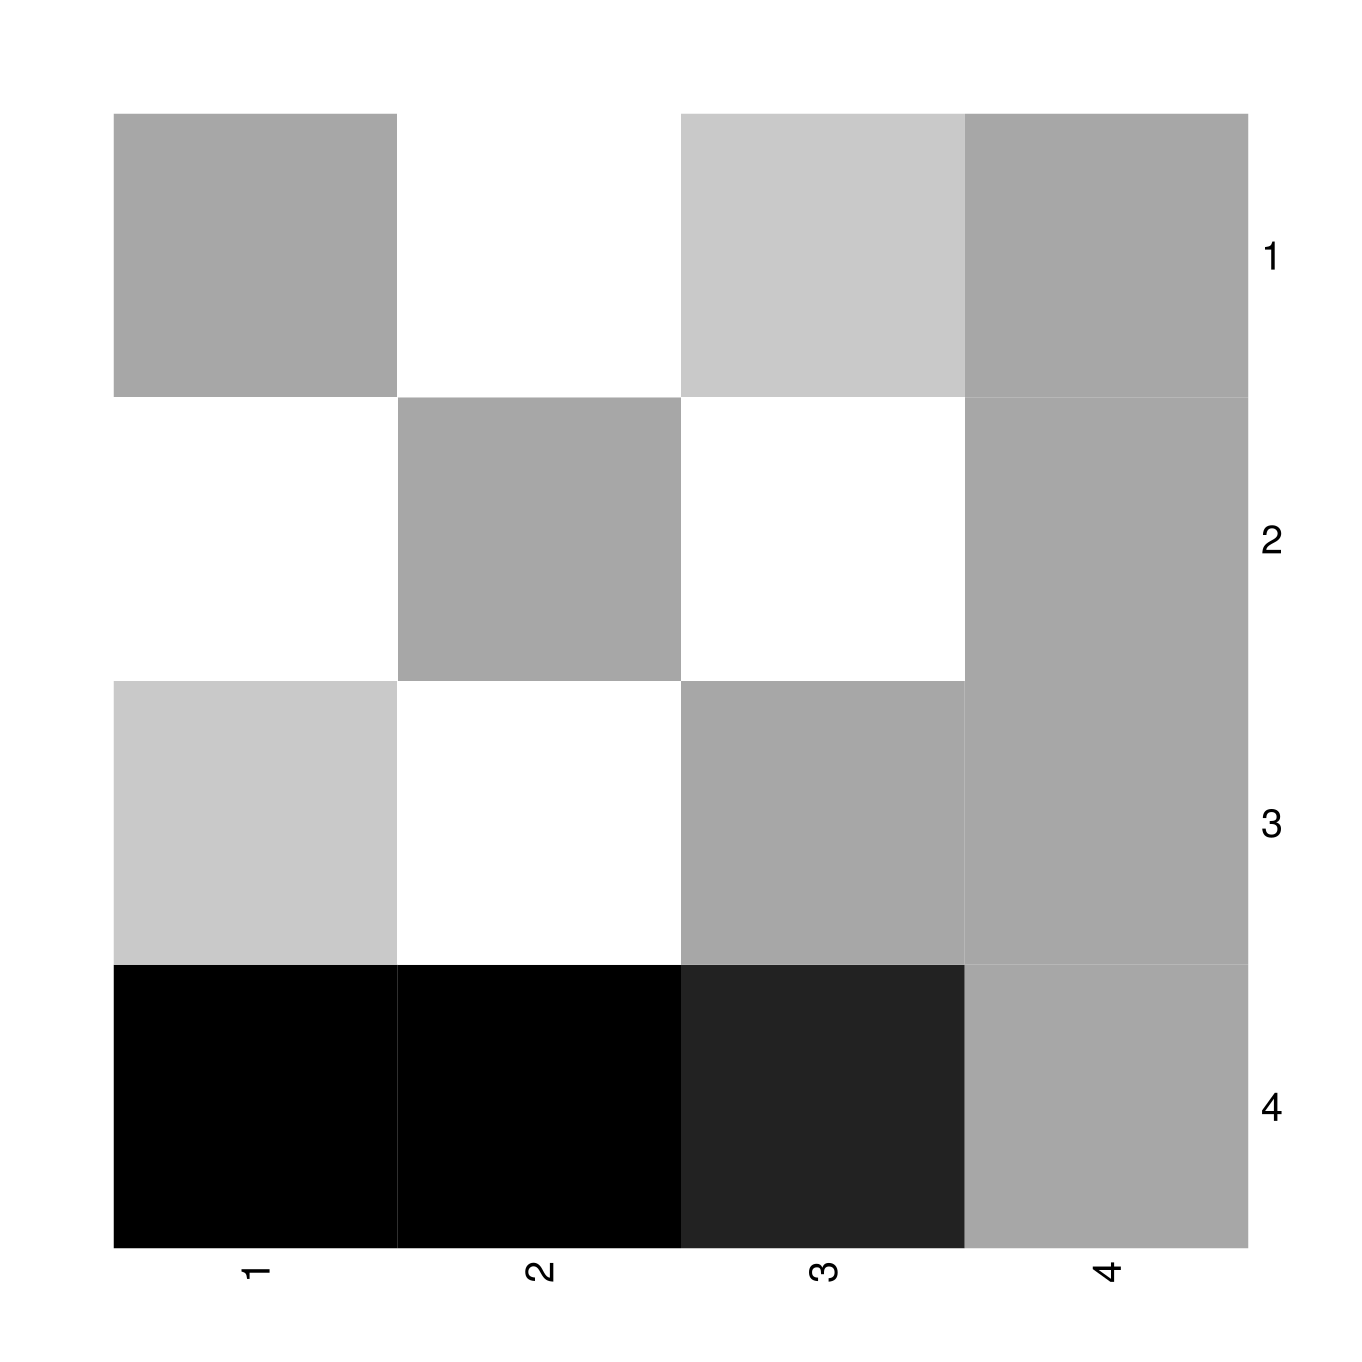
\includegraphics[width=0.8\textwidth]{isolet_bw}
                \caption{Isolet}
            \end{subfigure}
        \end{figure}

        \begin{itemize}
            \item\textbf{Identification des vues bruitées.}
            \item Apparition de \textbf{méta-clusters} (des clusters de 
                clusters). Les vues auront tendance à se regrouper en 
                sous-groupe mutuellement d'accord.
        \end{itemize}
    \end{frame}

    \begin{frame}{Optimisation des paramètres: résumé}
        \begin{itemize}
            \item Proposition d'un \textbf{système de pondération automatique 
                des vues externes} pour le clustering collaboratif.\\~\\
            \item \textbf{Amélioration} de la valeur du critère collaboratif
            \item \textbf{Identification des vues bruitées}
            \item \textbf{(BONUS)} Apparition de \textbf{méta-clusters} de 
                vues\\~\\
        \end{itemize}

        \begin{center}
            \fontsize{14pt}{15pt}
            \onslide<2>{\textbf{Est-il possible d'étendre l'idée de 
                collaboration\\à d'autres problèmes que le clustering ?}
            }
        \end{center}
    \end{frame}

    \section{Système de reconstruction collaboratif}
    \begin{frame}
        \begin{figure}[b]
            \centering
            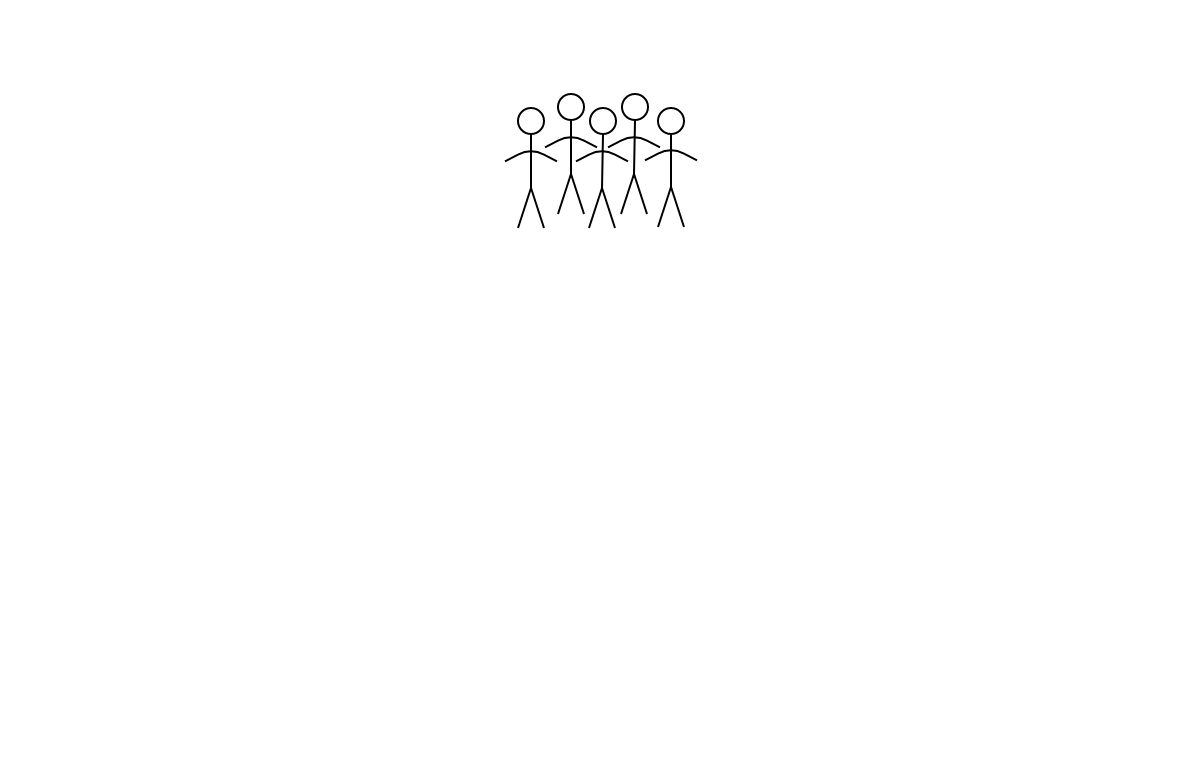
\includegraphics[scale=.26]{idee_reconstruction_collaborative1}
        \end{figure}
    \end{frame}

    \begin{frame}
        \begin{figure}[b]
            \centering
            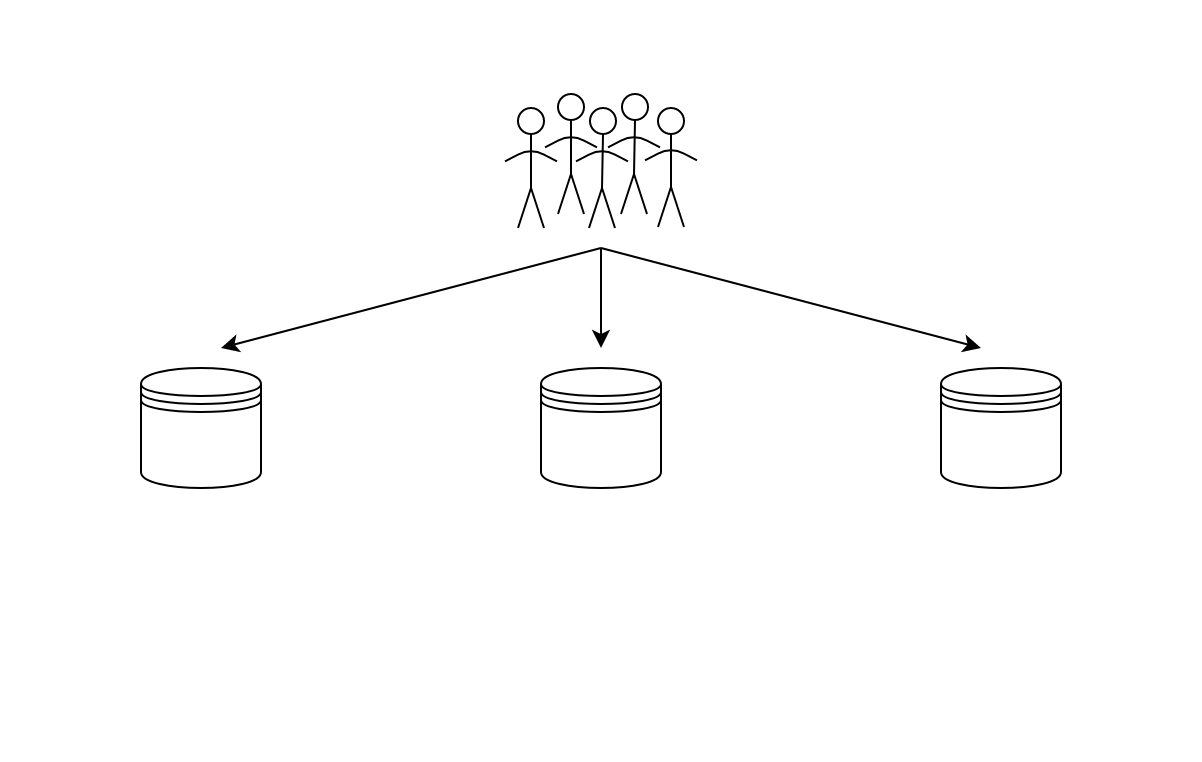
\includegraphics[scale=.26]{idee_reconstruction_collaborative2}
        \end{figure}
    \end{frame}

    \begin{frame}
        \begin{figure}[b]
            \centering
            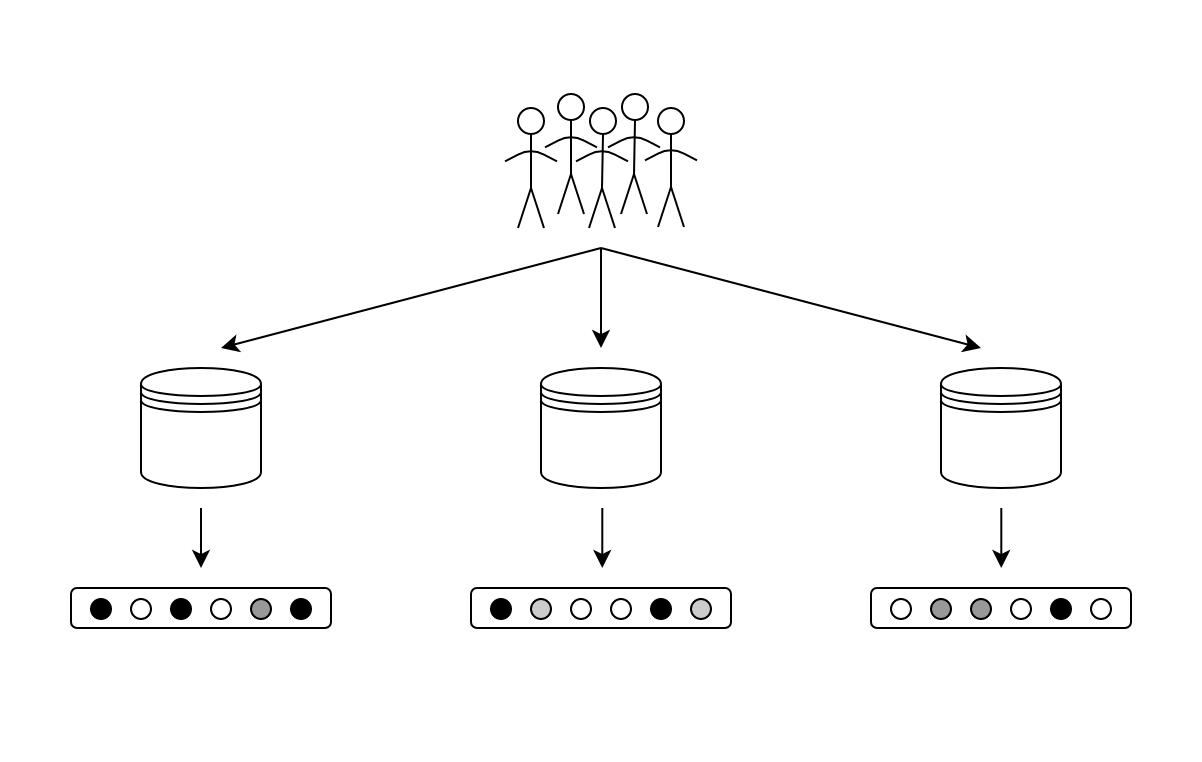
\includegraphics[scale=.26]{idee_reconstruction_collaborative3}
        \end{figure}
    \end{frame}

    \begin{frame}
        \begin{figure}[b]
            \centering
            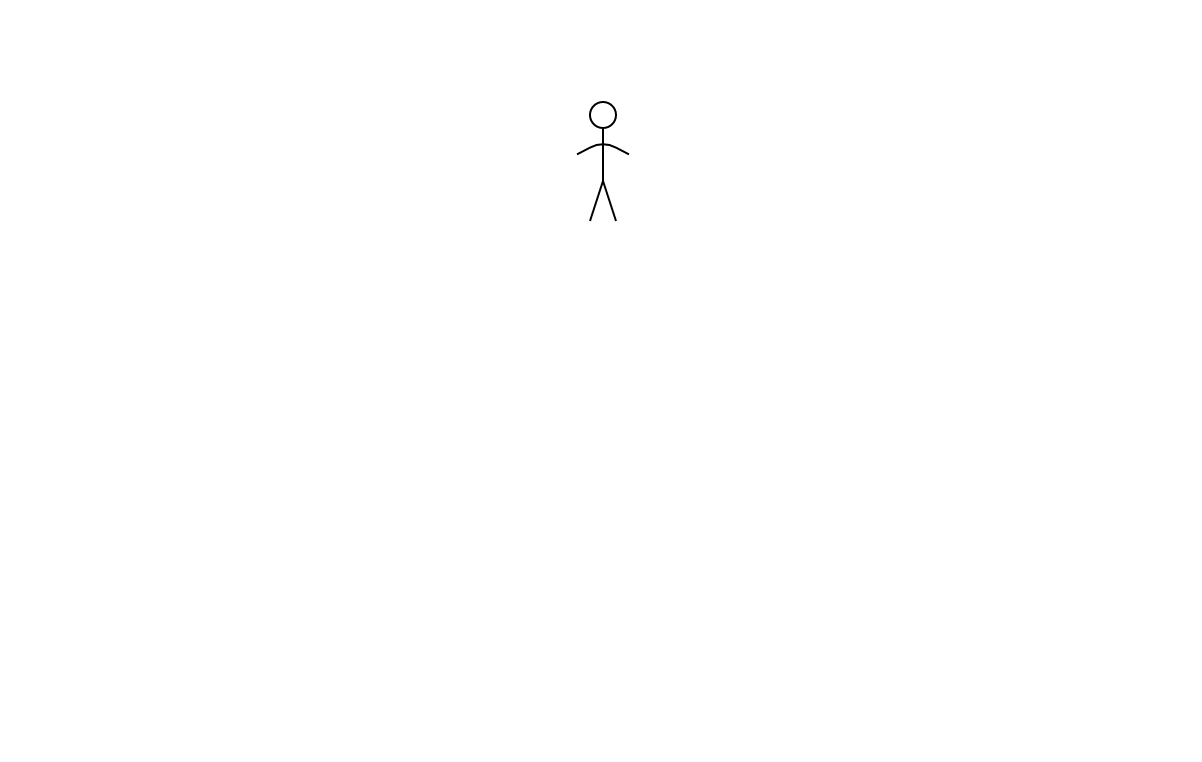
\includegraphics[scale=.26]{idee_reconstruction_collaborative4}
        \end{figure}
    \end{frame}

    \begin{frame}
        \begin{figure}[b]
            \centering
            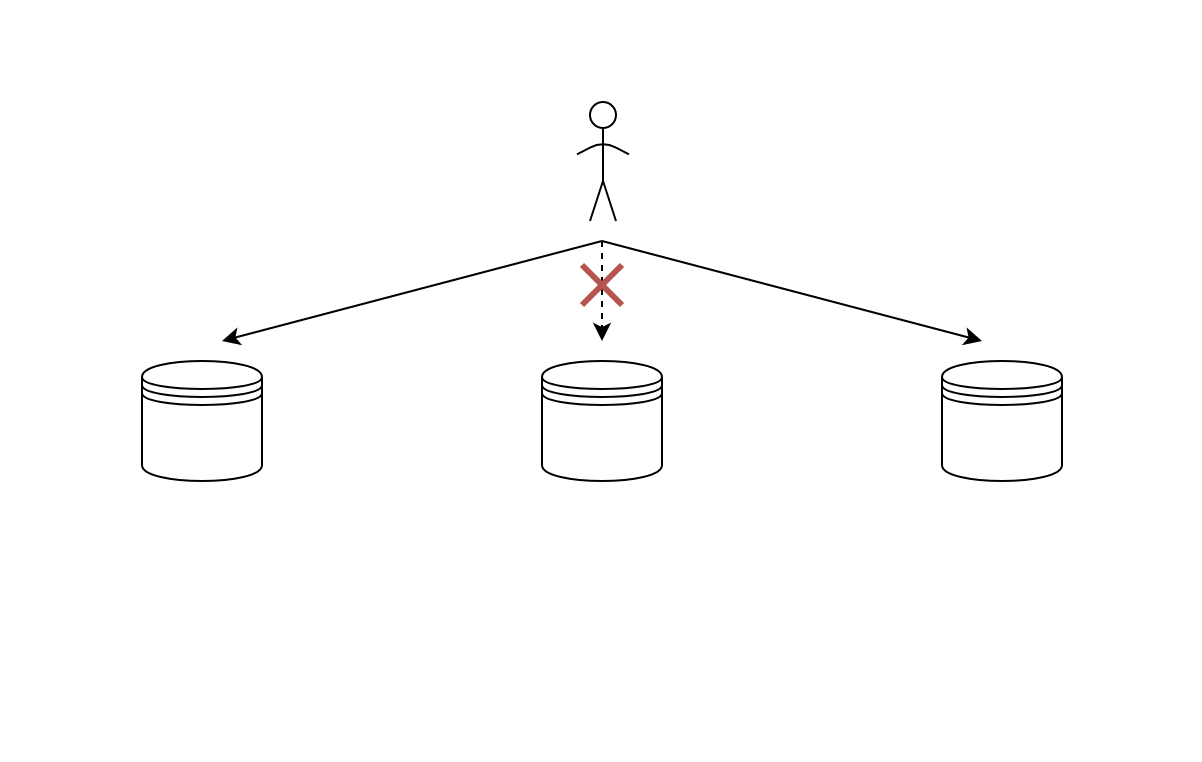
\includegraphics[scale=.26]{idee_reconstruction_collaborative5}
        \end{figure}
    \end{frame}

    \begin{frame}
        \begin{figure}[b]
            \centering
            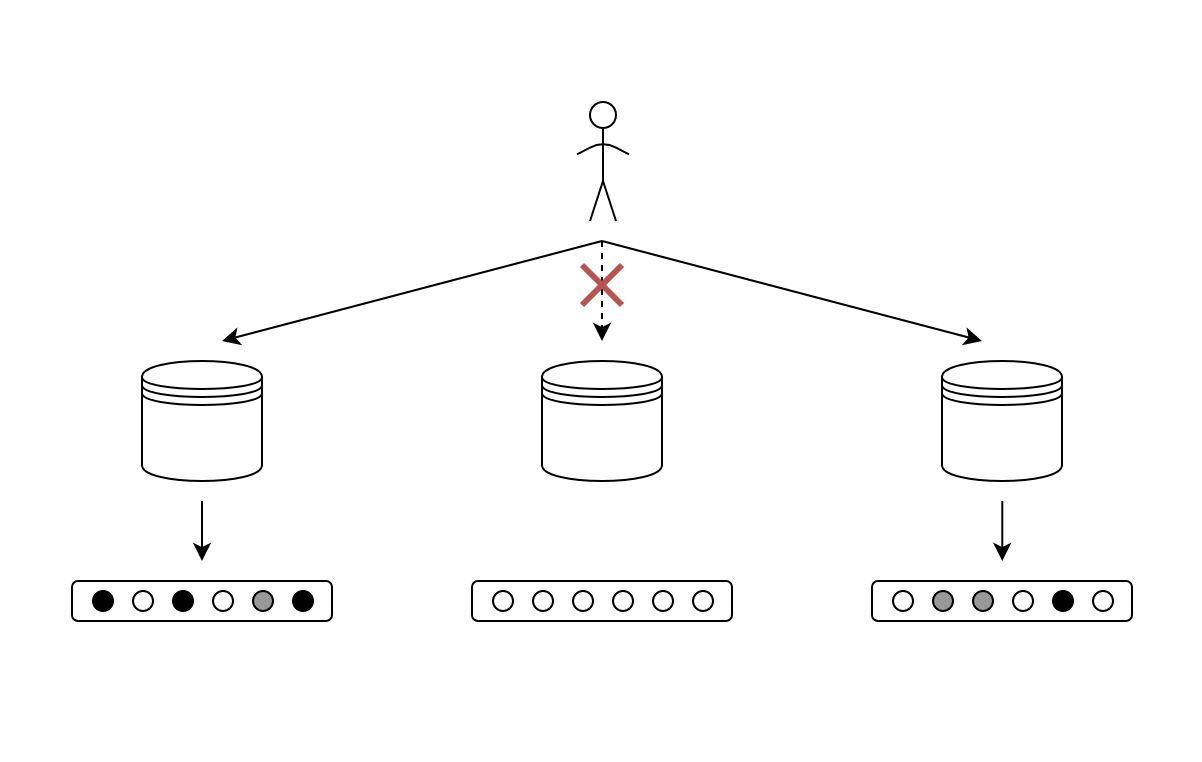
\includegraphics[scale=.26]{idee_reconstruction_collaborative6}
        \end{figure}
    \end{frame}

    \begin{frame}
        \begin{figure}[b]
            \centering
            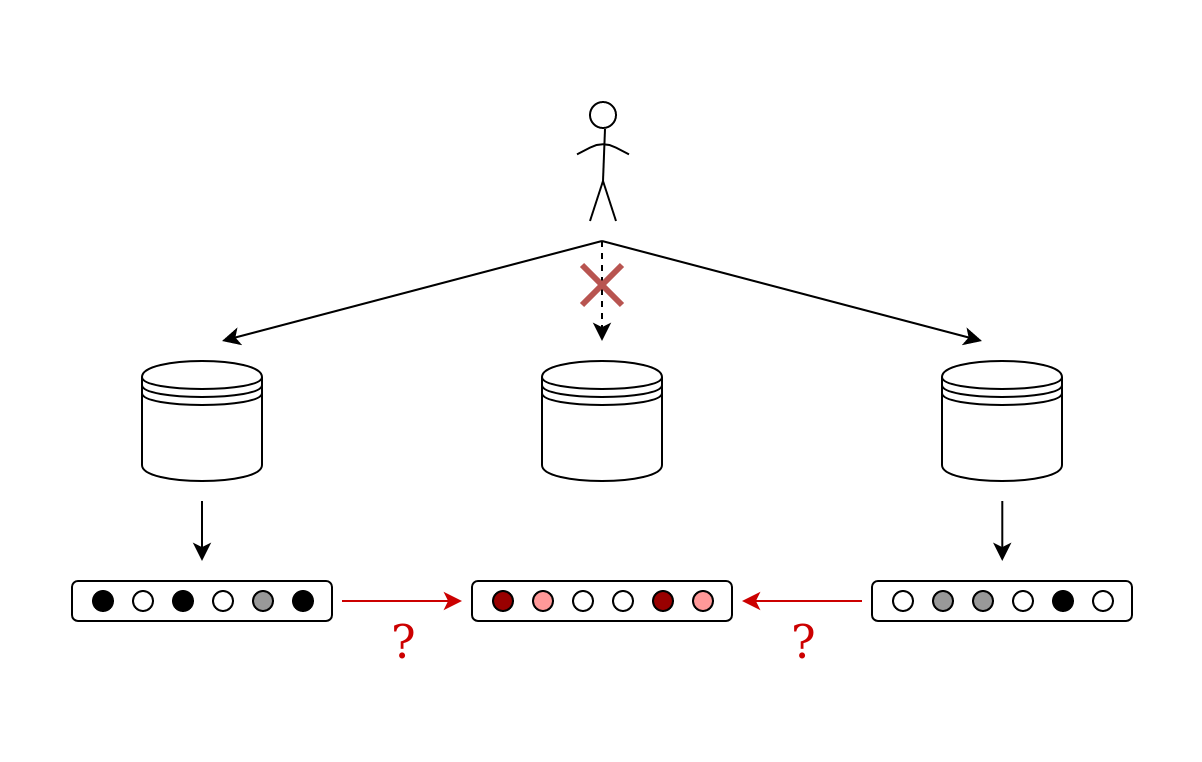
\includegraphics[scale=.26]{idee_reconstruction_collaborative7}
        \end{figure}
    \end{frame}

    \begin{frame}{Reconstruction collaborative: définition}
        \textbf{Objectif 1}: \textbf{Reconstruire localement} une approximation 
        de l'individu manquant à partir des informations présentes dans 
        \textbf{les vues externes}.\\~\\
        \textbf{Objectif 2}: Effectuer \textbf{une classification} des individus 
        reconstruits et \textbf{comparer} avec les résultats obtenus sur les 
        \textbf{données originales}.
        \vspace{0.5cm}
        \begin{figure}[h]
            \centering
            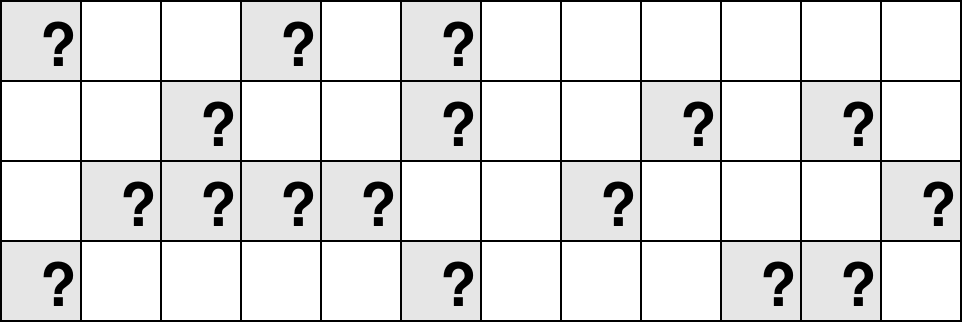
\includegraphics[scale=.15]{missing}
        \end{figure}
    \end{frame}

    \begin{frame}{Reconstruction collaborative: défis}
        \begin{enumerate}
            \item \textbf{Compresser et anonymiser} les données
            \item \textbf{Transférer de l'information} d'une vue externe à une 
                vue locale
            \item \textbf{Combiner les informations} en provenance de 
                différentes sources
        \end{enumerate}

        \onslide<2->{Ce que nous proposons:}
        \begin{enumerate}[<+(1)->]
            \item \textbf{Des réseaux de neurones} (autoencodeurs).
            \item \textbf{D'autres réseaux de neurones} (perceptrons 
                multi-couches).
            \item \textbf{Une nouvelle méthode de combinaison}.
        \end{enumerate}
    \end{frame}

    \begin{frame}{Réseaux de neurones}
        \begin{columns}
            \begin{column}{0.4\textwidth}
                \begin{itemize}
                    \item Réseau de neurone: \textbf{approximateur universel de 
                        fonction}.\\~\\
                    \item \textbf{Backpropagation}: Méthode utilisée pour 
                        \textbf{mettre à jour des paramètres}.\\~\\
                    \item L'erreur est propagée \textbf{de la sortie vers l'entrée} du 
                        réseau.
                \end{itemize}
            \end{column}
            \begin{column}{0.6\textwidth}
                \begin{figure}[h]
                    \centering
                    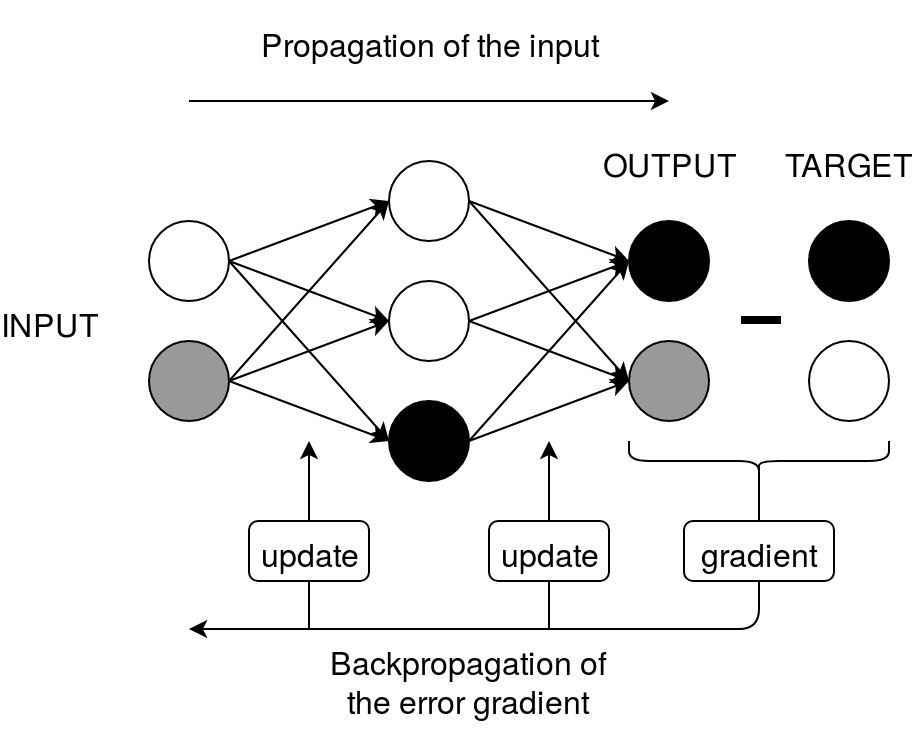
\includegraphics[scale=.20]{backprop}
                \end{figure}
            \end{column}
        \end{columns}
    \end{frame}

    \begin{frame}{Réseaux de neurones: MLP et autoencodeurs}
        \begin{columns}
            \begin{column}{0.5\textwidth}
                Perceptron multi-couches
                \begin{itemize}
                    \item entrées et sorties \textbf{différentes}
                    \item apprentissage \textbf{supervisé}
                \end{itemize}
                \begin{figure}[h]
                    \centering
                    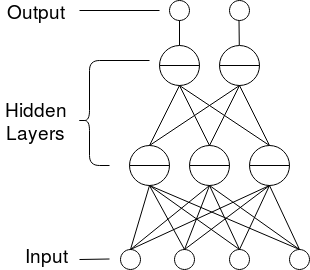
\includegraphics[scale=.18]{mlp}
                \end{figure}
            \end{column}
            \begin{column}{0.5 \textwidth}
                Autoencodeur
                \begin{itemize}
                    \item entrées et sorties \textbf{identiques}
                    \item apprentissage \textbf{non supervisé}
                \end{itemize}
                \begin{figure}[h]
                    \centering
                    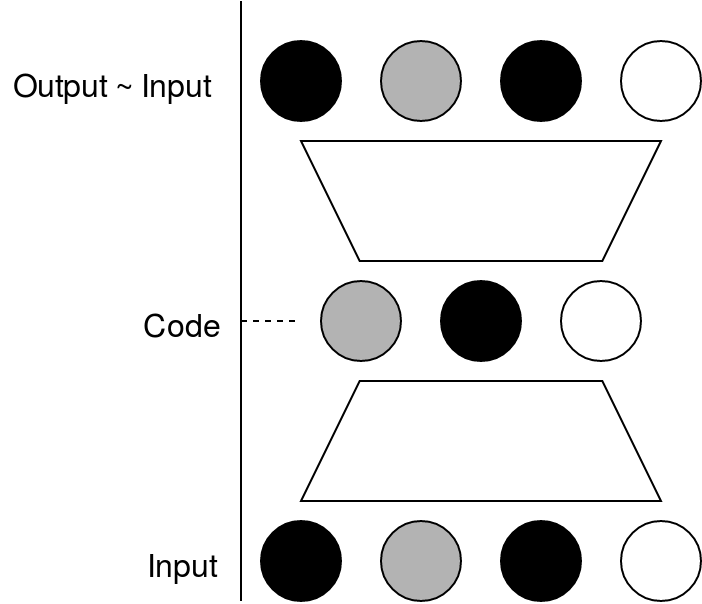
\includegraphics[scale=.18]{ae}
                \end{figure}
            \end{column}
        \end{columns}
    \end{frame}

    \begin{frame}{Reconstruction collaborative: rappel}
        Rappel de la problèmatique
        \begin{itemize}
            \item Un individu décrit dans \textbf{toutes les vues sauf une}
            \item Utilisation des informations externes pour obtenir \textbf{une 
                approximation locale}
        \end{itemize}
        \vspace{-0.5cm}
        \begin{figure}[b]
            \centering
            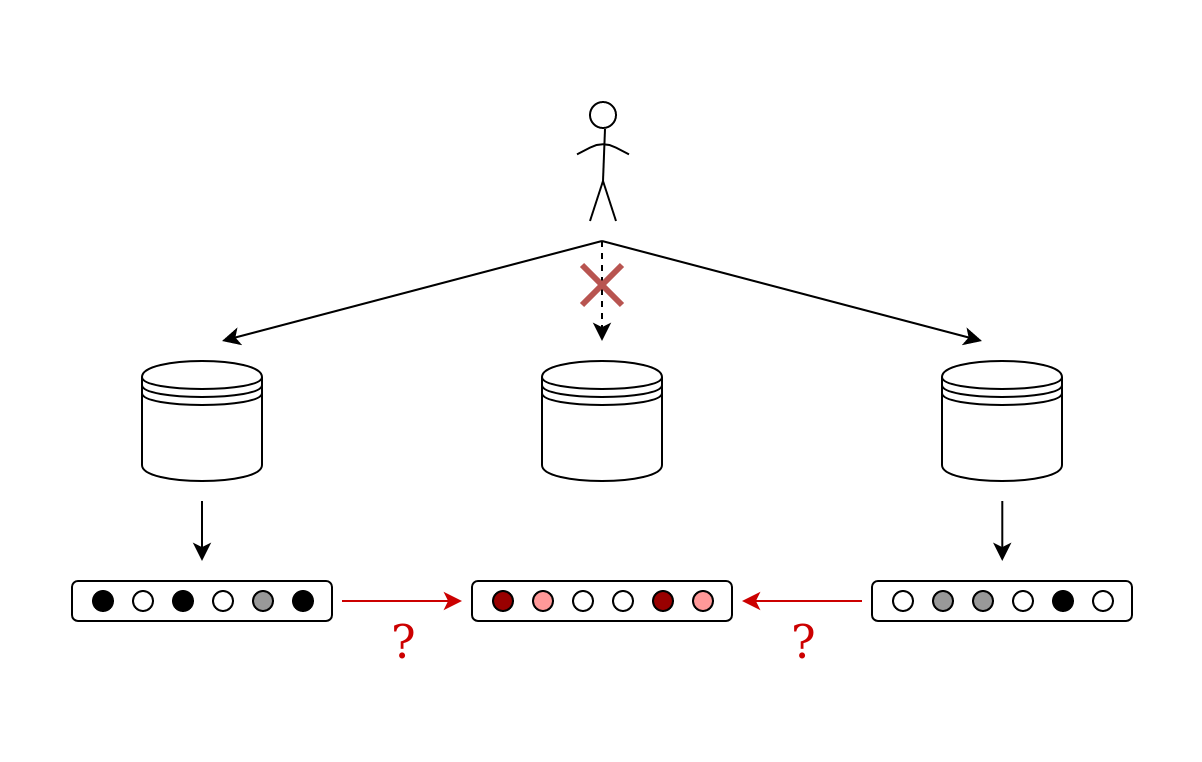
\includegraphics[scale=.21]{idee_reconstruction_collaborative7}
        \end{figure}
    \end{frame}

    \begin{frame}{Reconstruction collaborative: système}
        \begin{figure}[h]
            \centering
            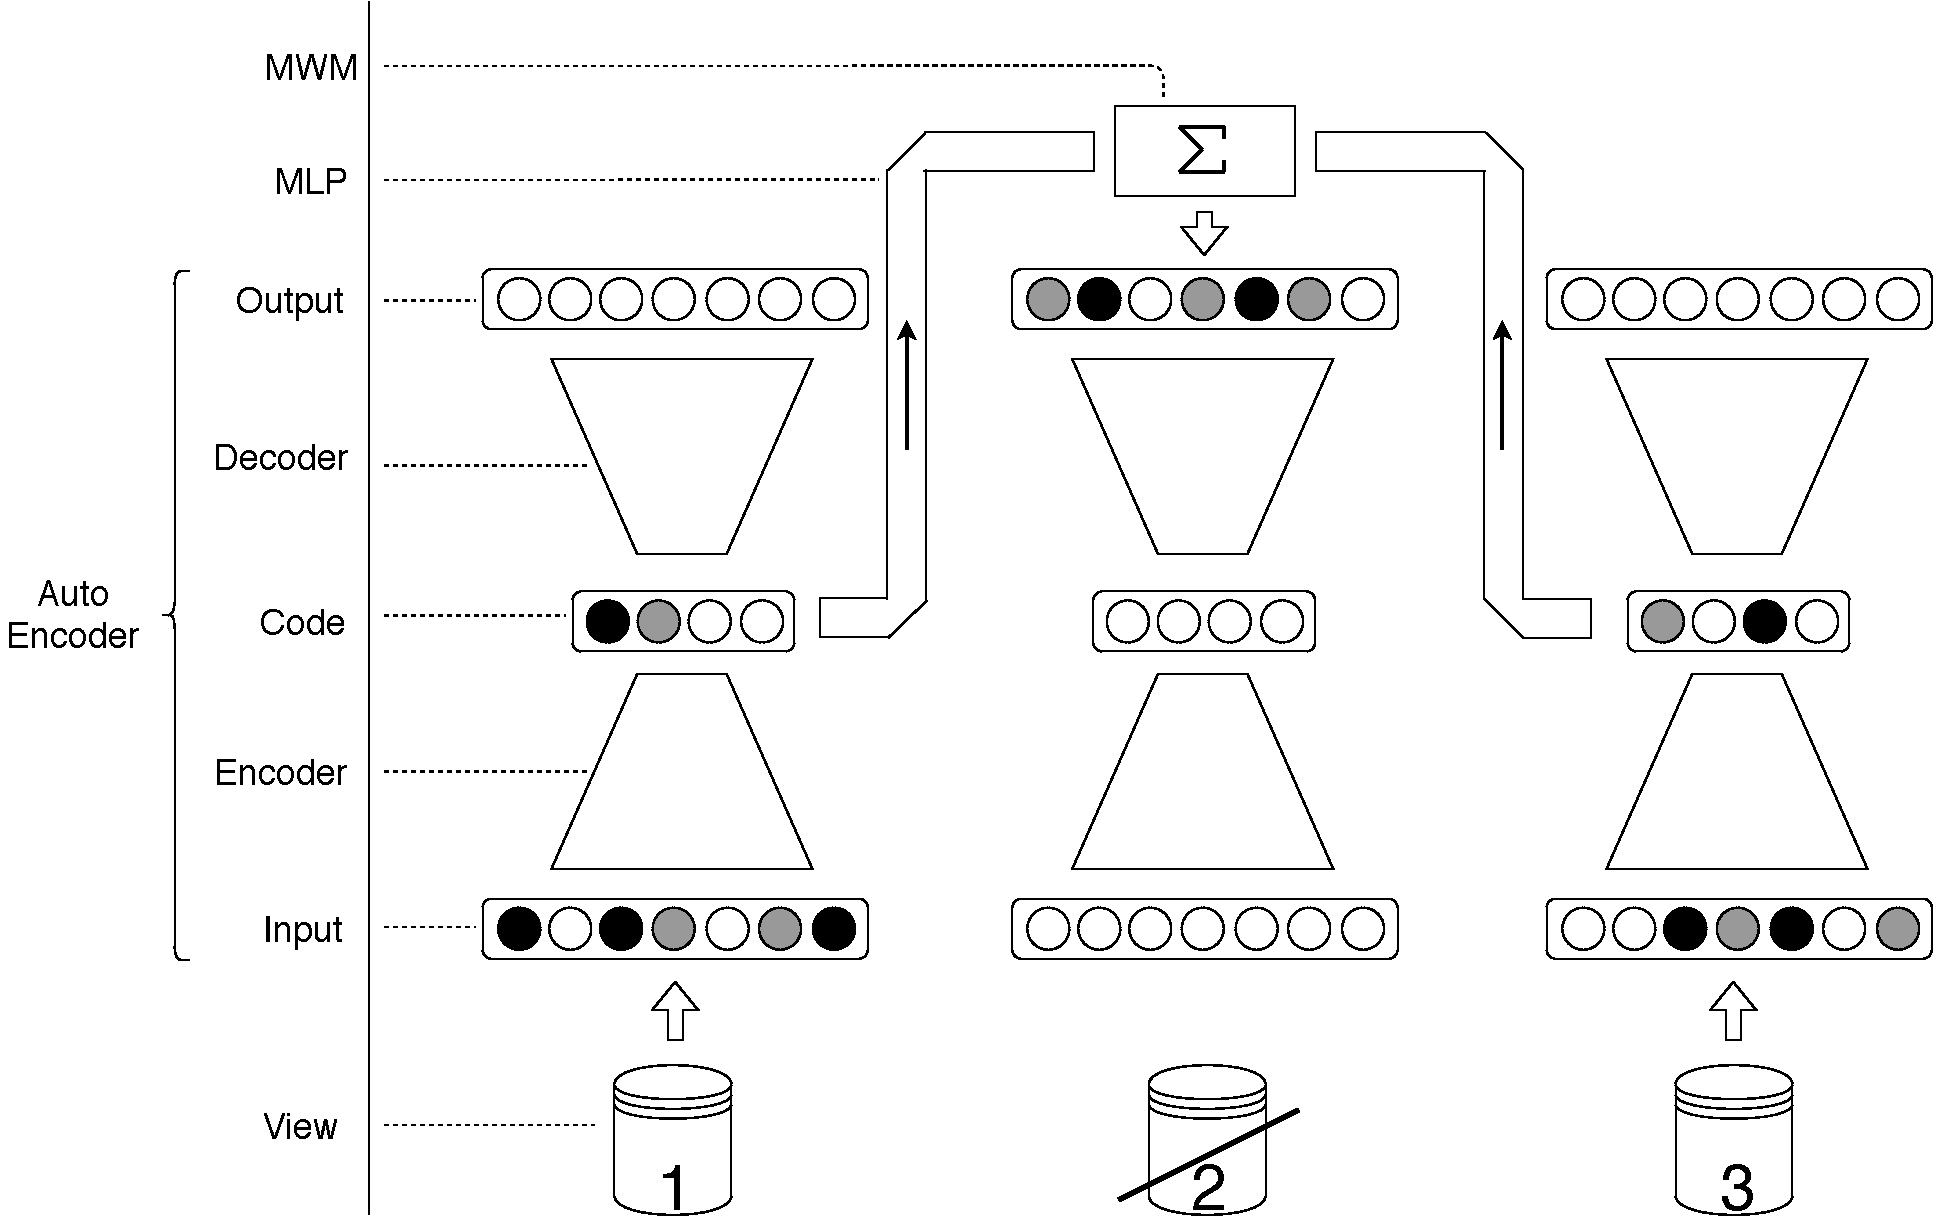
\includegraphics[scale=.28]{base_system.pdf}
            \caption{Architecture d'un système de reconstruction collaborative}
        \end{figure}
    \end{frame}

    \begin{frame}{Reconstruction collaborative: système}
        \begin{columns}
            \fontsize{10pt}{12pt}
            \begin{column}{0.5\textwidth}
                \textbf{Autoencodeurs}
                \begin{itemize}
                    \item Un par vue: encoder chaque espace
                    \item Rend difficile la reconstruction des données 
                        originales sans le décodeur
                \end{itemize}
            \end{column}
            \begin{column}{0.5\textwidth}
                \textbf{Perceptron multi-couches}
                \begin{itemize}
                    \item Décode les représentations externes
                    \item Passe d'un espace codé à l'espace local
                \end{itemize}
            \end{column}
        \end{columns}
        \vspace{-0.3cm}
        \begin{figure}[h]
            \centering
            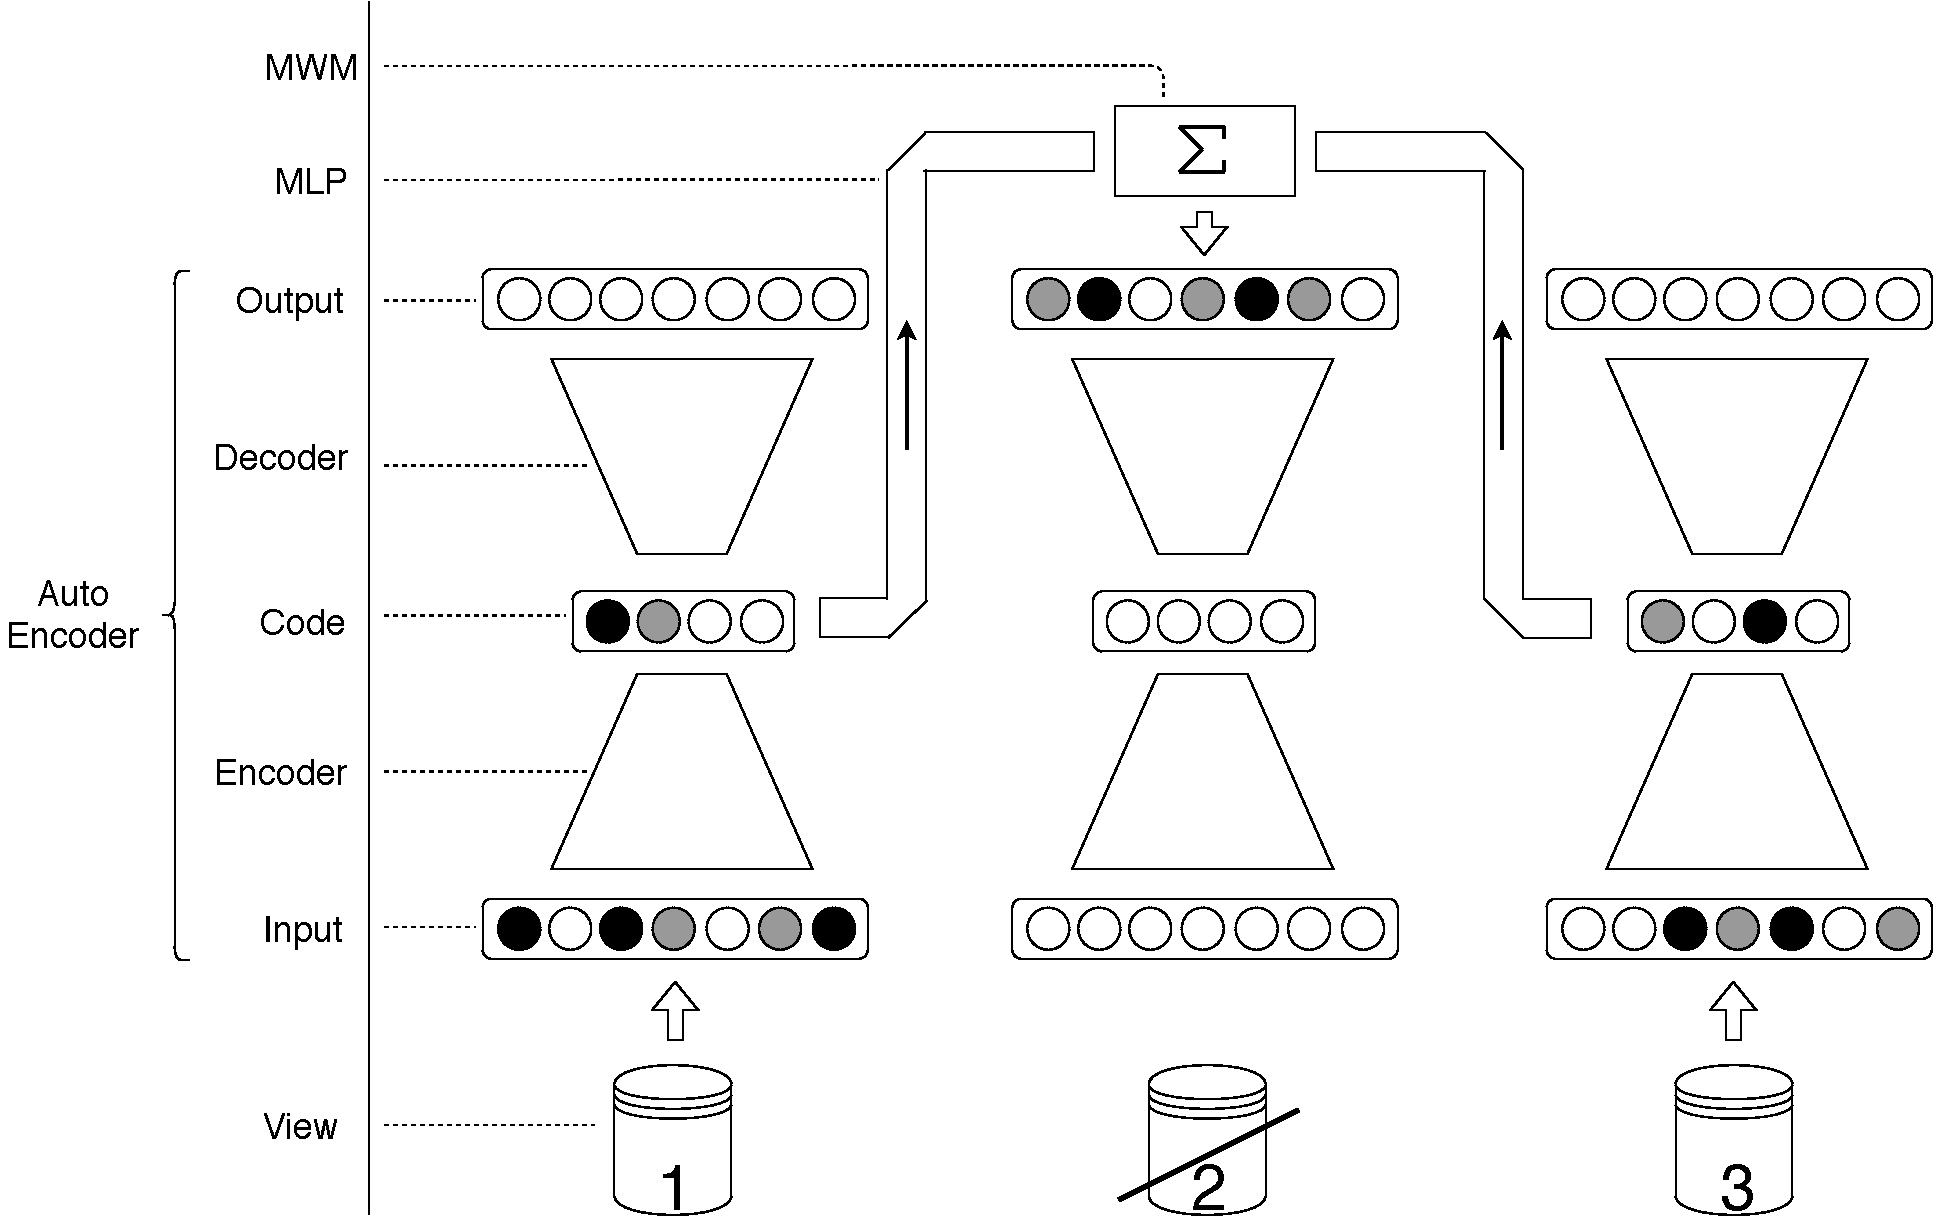
\includegraphics[scale=.23]{base_system.pdf}
        \end{figure}
        \vspace{-0.3cm}
    \end{frame}

    \begin{frame}{Reconstruction collaborative: combinaison}
        \begin{itemize}
            \item<+-> Pour chaque individu et avec $N$ vues, on peut avoir 
                jusqu'à $N-1$ \textbf{reconstructions différentes}.
            \item<.-> Comment les combiner ?\\~\\
            \item<+-> Habituellement, combinaison \textbf{pondérée} des 
                différentes reconstructions.
                \begin{itemize}
                    \item Un scalaire par vue
                    \item Différentes façons d'apprendre les poids\\~\\
                \end{itemize}
            \item<+-> \textit{MAIS} hypothèse forte: chaque vue contient 
                exactement \textbf{la même information} sur chaque descripteur 
                $\rightarrow$ irréaliste.
            \item<.-> À la place d'un poids unique, nous utilisons un 
                \textbf{masque}.
        \end{itemize}
    \end{frame}

    \begin{frame}{Reconstruction collaborative: combinaison}
        \begin{itemize}
            \item Chaque vue possède $N-1$ masques, un par vue externe, utilisés 
                pour \textbf{pondérer chaque représentation externe}.
            \item Chaque masque est entraîné de manière itérative
            \item \textbf{Avantage}: les masques peuvent se concentrer sur 
                \textbf{les parties les mieux reconstruites} par la vue externe.
        \end{itemize}
        \begin{figure}[b]
            \centering
            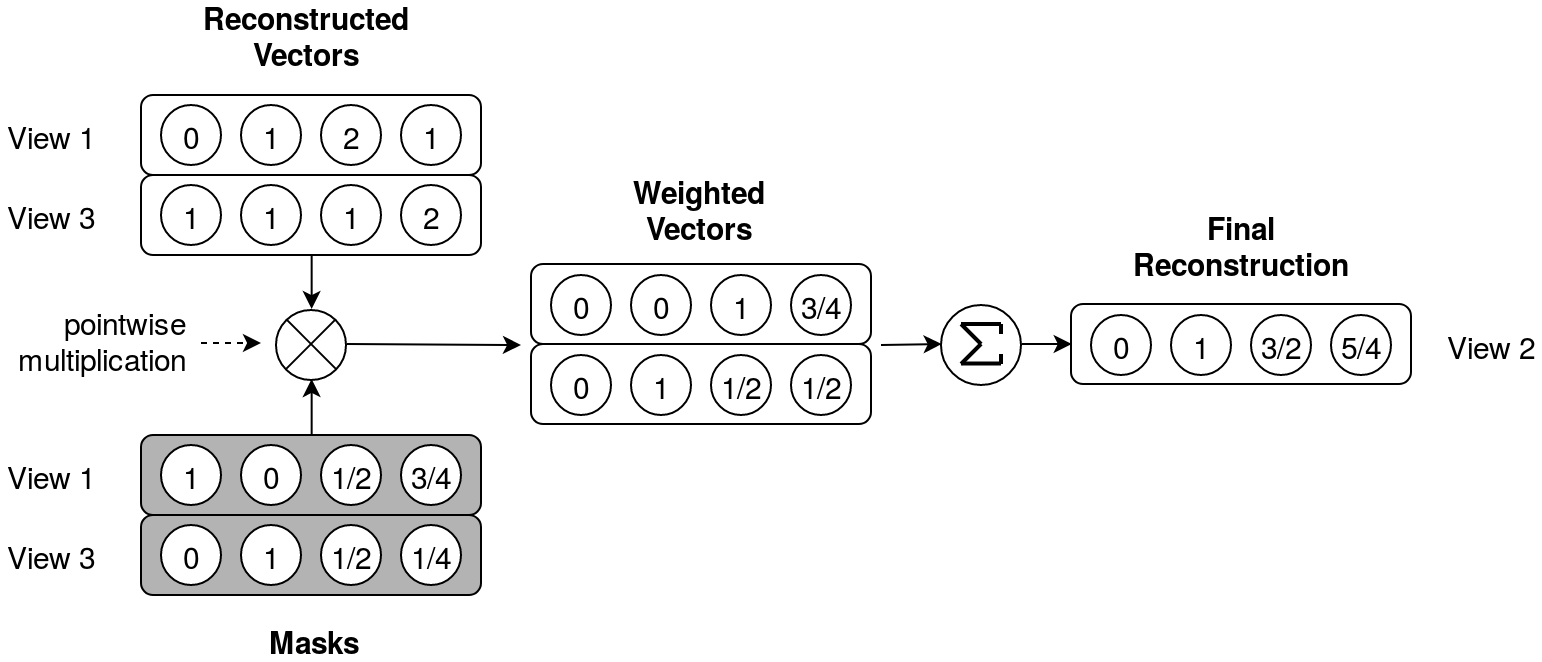
\includegraphics[scale=.17]{mwm.png}
            \caption{Pondération par masque (Masked Weighting Method
                (\textbf{MWM}) en anglais).
            }
        \end{figure}
    \end{frame}

    \begin{frame}{Reconstruction collaborative: combinaison}
        Idée de base pour la mise à jour des poids
        \begin{equation*}
             E_i = \frac{1}{|V_i|}\sum_{x_i \in V_i}||x_i - \widetilde{x}_i||^2 
             \quad puis \quad \frac{\partial E_i}{\partial w_{i|j}^k} = 0
        \end{equation*}
        \begin{itemize}
            \item $E_i$ = erreur de la $i$-ème vue
            \item $V_i$ = $i$-ème vue
            \item $x_i$ = individu de $V_i$
            \item $w_{i|j}^k$ = $k$-ème coordonnée du masque attribué à la 
                $j$-ème vue
        \end{itemize}
    \end{frame}

    \begin{frame}{Reconstruction collaborative: combinaison}
        Après calcul:
        \begin{equation*}
            w_{i|j}^k = \frac{\sum_{x_i \in V_i} x_{i|j}^k\big(x_i^k - 
                    \only<1>{\sum_{j'\in[1..N]\backslash \{i,j\}} w_{i|j'}^k 
                    x_{i|j'}^k}\only<2>{\textcolor{red}{ 
                    \sum_{j'\in[1..N]\backslash \{i,j\}} w_{i|j'}^k} x_{i|j'}^k}
            \big)}{\sum_{x_i \in V_i}(x_{i|j}^k)^2}
        \end{equation*}
        \begin{itemize}
            \item<2> La mise à jour d'un poids dépend de \textbf{tous les autres 
                paramètres}\\$\rightarrow$ Définition d'une règle de mise à jour 
                \textbf{itérative}.
        \end{itemize}
    \end{frame}

    \begin{frame}{Reconstruction collaborative: entraînement}
        \begin{itemize}
            \item Entraînement \textbf{séquentiel}
                \begin{itemize}
                    \item les autoencodeurs pour \textbf{encoder} les données
                    \item les perceptrons multi couches pour 
                        \textbf{reconstruire} les individus
                    \item les masques pour \textbf{combiner} les échantillons 
                        reconstruits\\~\\
                \end{itemize}
            \item Une vue n'a \textbf{\textit{jamais}} accès aux données 
                originales de deux vues différentes.
                \begin{itemize}
                    \item \textbf{autoencodeurs}: données originales locales
                    \item \textbf{perceptrons}: données externes encodées + 
                        données originales locales
                    \item \textbf{masques}: échantillons reconstruits + données 
                        originales locales
                \end{itemize}
        \end{itemize}
    \end{frame}

    \begin{frame}{Reconstruction collaborative: expériences}
        \begin{itemize}
            \item Wisconsin Diagnostic Breast Cancer (WDBC)
                \begin{itemize}
                    \item 569 individus
                    \item 30 descripteurs répartis en 3 vues
                \end{itemize}
            \item Multi-Features Digital Dataset (MFDD)
                \begin{itemize}
                    \item 2000 individus
                    \begin{itemize}
                        \item 76 coefficients de Fourier
                        \item 216 correlations profile
                        \item 64 coefficients Karhunen-Love
                        \item\textbf{240 pixels moyennés en fenêtres de 2 
                            $\times$ 3}
                        \item 47 moments de Zernike
                    \end{itemize}
                \end{itemize}
            \item Madelon
                \begin{itemize}
                    \item 4400 individus
                    \item 20 (utiles) 480 (bruits) variables
                \end{itemize}
        \end{itemize}
    \end{frame}

    \begin{frame}{Reconstruction collaborative: critères}
        \begin{itemize}
            \item Distance quadratique moyenne
                \begin{equation*}
                    MSE(x, y) = \frac{1}{K}\sum_{i = 1}^{K}(x_i - y_i)^2
                \end{equation*}
            \item Différence relative moyenne
                \begin{equation*}
                    MRD(X, Y) = \frac{1}{K}\sum_{i=1}^{K}\Big|\frac{x_i - y_i}{y_i}\Big|
                \end{equation*}
            \item Analyse visuelle d'images reconstruites (MFDD)
        \end{itemize}
    \end{frame}

    \begin{frame}{Reconstruction collaborative: résultats}
        \begin{figure}[!h]
            \centering
            \begin{subfigure}[c]{0.45\textwidth}
                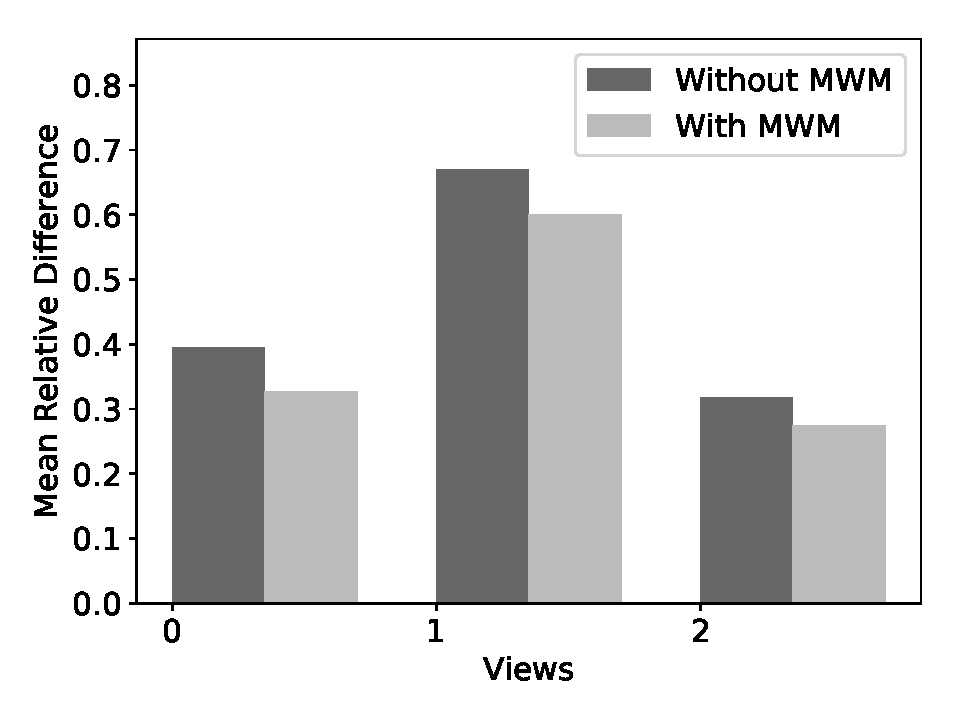
\includegraphics[scale=.26]{mrd_wdbc}
                \caption{WDBC}
            \end{subfigure}
            \begin{subfigure}[c]{0.45\textwidth}
                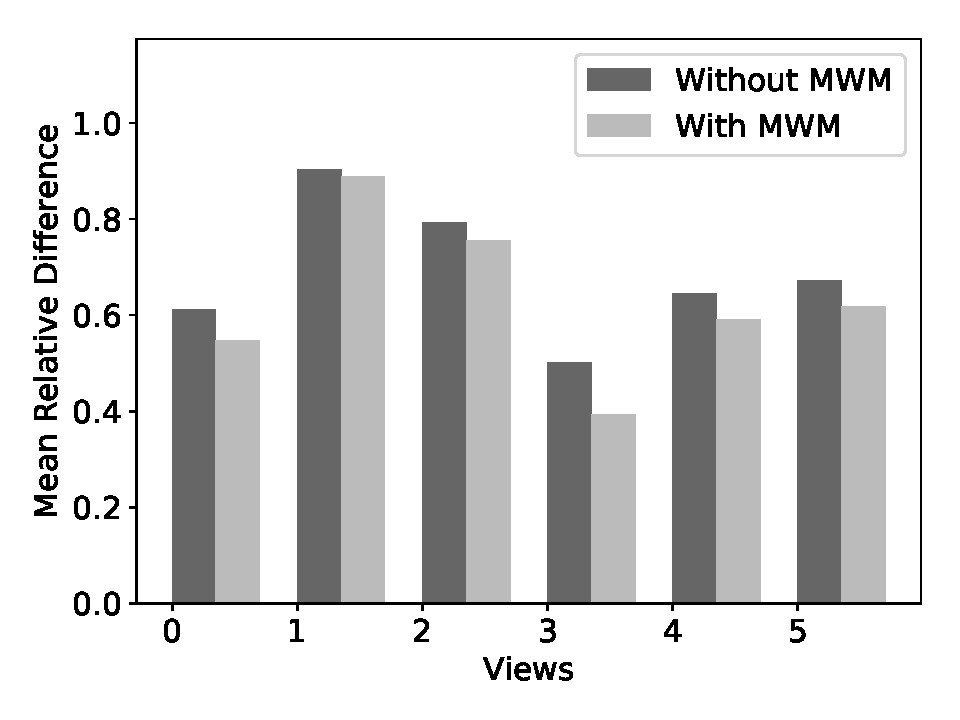
\includegraphics[scale=.26]{mrd_mfeat}
                \caption{MFDD}
            \end{subfigure}\\
            \begin{subfigure}[c]{0.45\textwidth}
                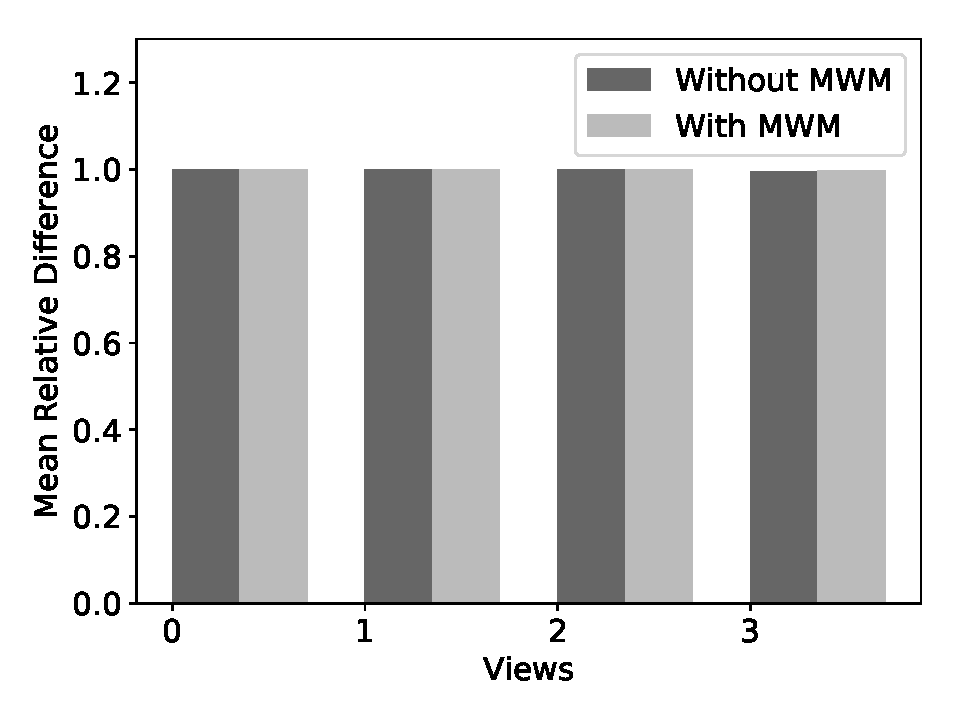
\includegraphics[scale=.26]{mrd_madelon}
                \caption{Madelon}
            \end{subfigure}
            \caption{Erreur par vue et par jeu de données}
        \end{figure}
    \end{frame}

    %\begin{frame}{Reconstruction collaborative: résultats}
        %\begin{figure}[!h]
            %\centering
            %\begin{subfigure}[c]{0.32\textwidth}
                %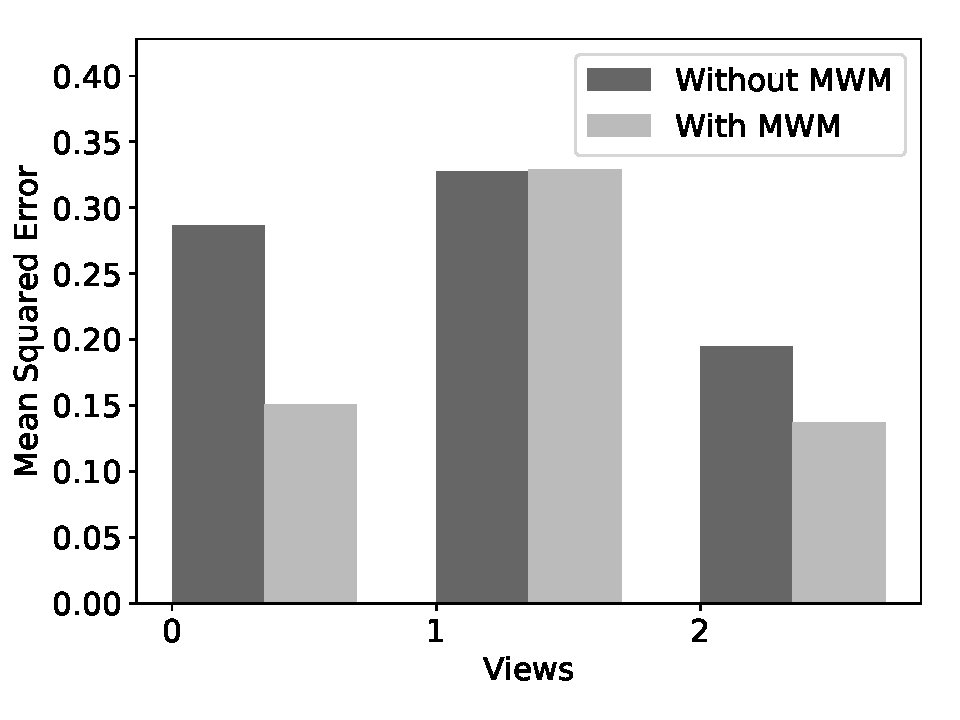
\includegraphics[scale=.21]{mse_wdbc}
            %\end{subfigure}
            %\begin{subfigure}[c]{0.32\textwidth}
                %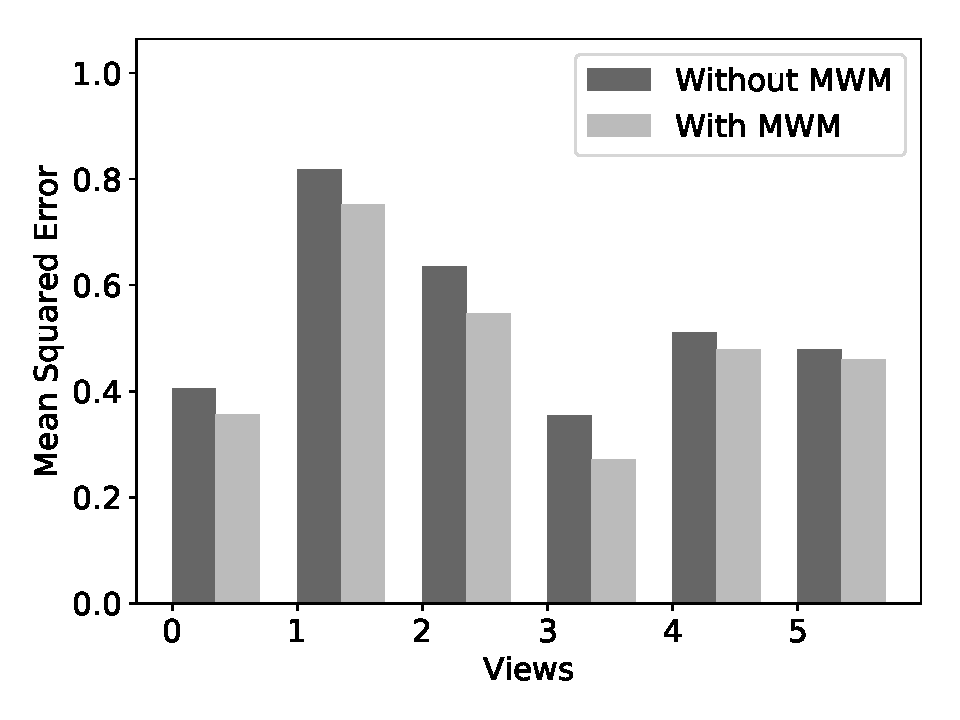
\includegraphics[scale=.21]{mse_mfeat}
            %\end{subfigure}
            %\begin{subfigure}[c]{0.32\textwidth}
                %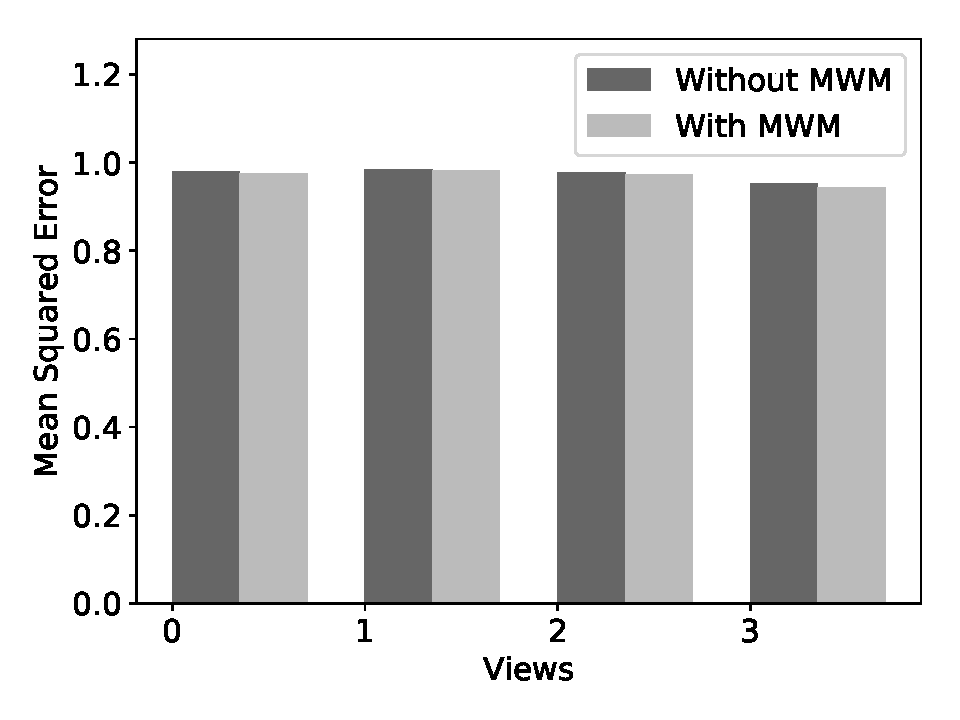
\includegraphics[scale=.21]{mse_madelon}
            %\end{subfigure}
            %\\
            %\begin{subfigure}[c]{0.32\textwidth}
                %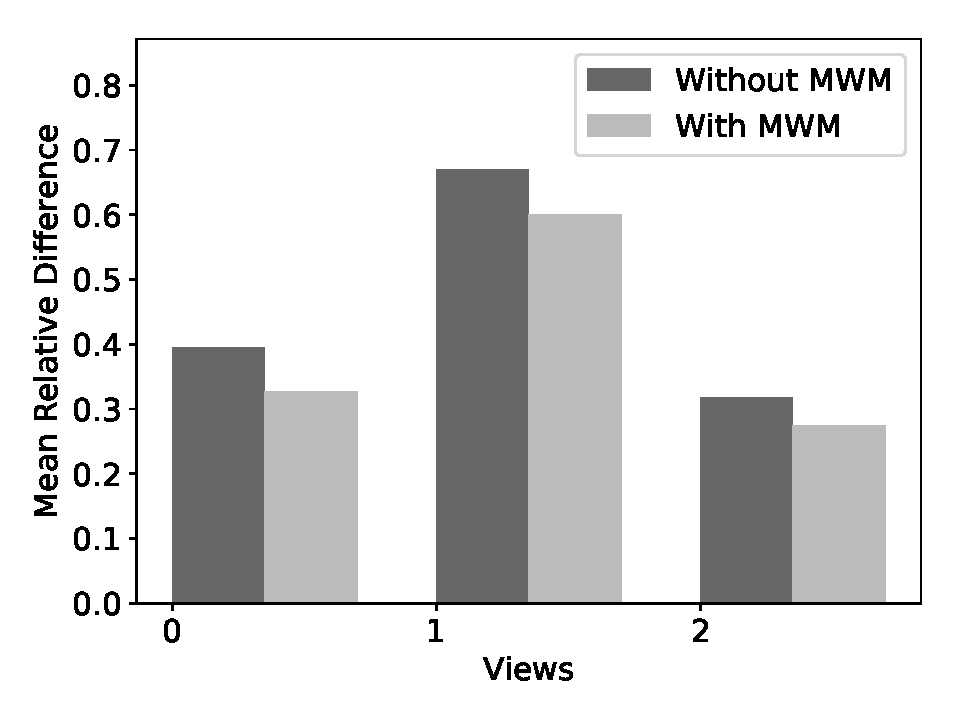
\includegraphics[scale=.21]{mrd_wdbc}
                %\caption{WDBC}
            %\end{subfigure}
            %\begin{subfigure}[c]{0.32\textwidth}
                %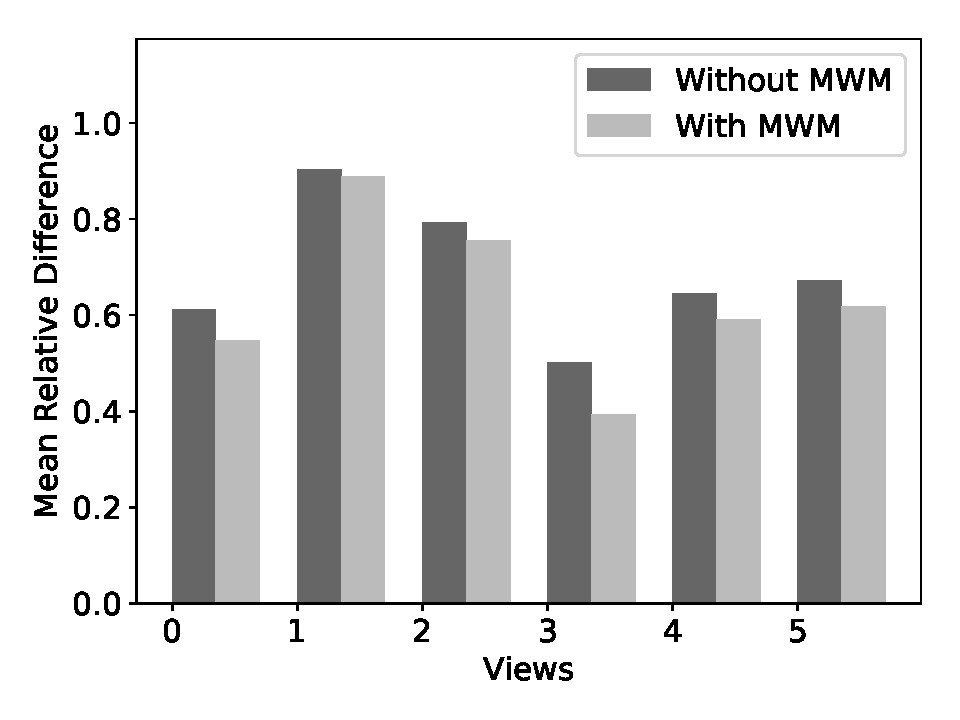
\includegraphics[scale=.21]{mrd_mfeat}
                %\caption{MFDD}
            %\end{subfigure}
            %\begin{subfigure}[c]{0.32\textwidth}
                %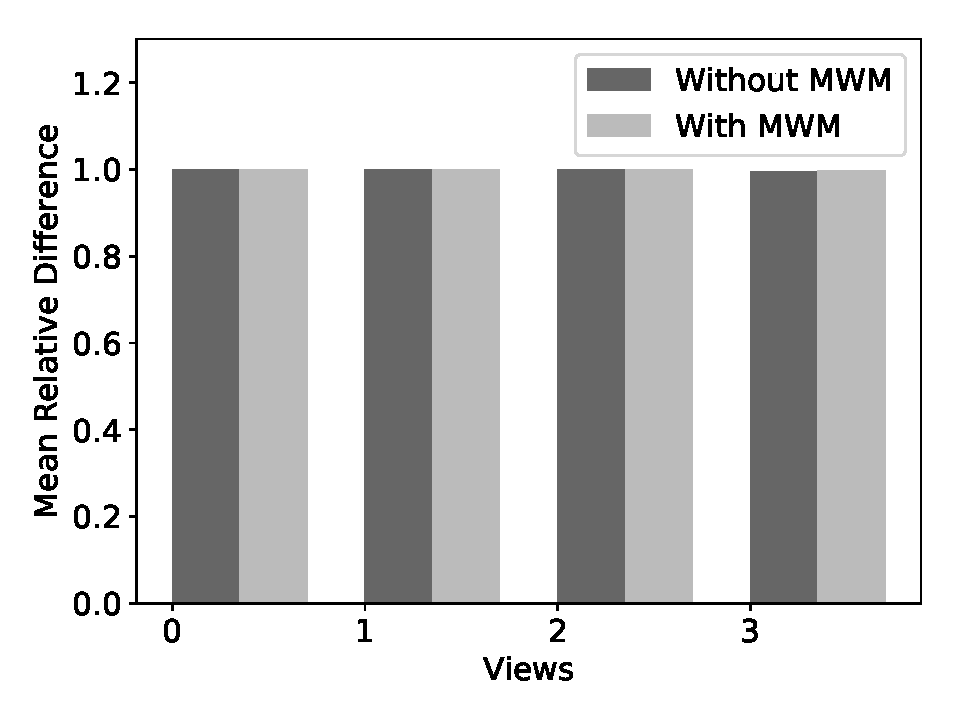
\includegraphics[scale=.21]{mrd_madelon}
                %\caption{Madelon}
            %\end{subfigure}
            %\caption{Erreur par vue et par jeu de données}
        %\end{figure}
    %\end{frame}

    \begin{frame}{Reconstruction collaborative: images originales}
        \begin{figure}[h]
            \centering
            \begin{subfigure}[c]{0.18\textwidth}
                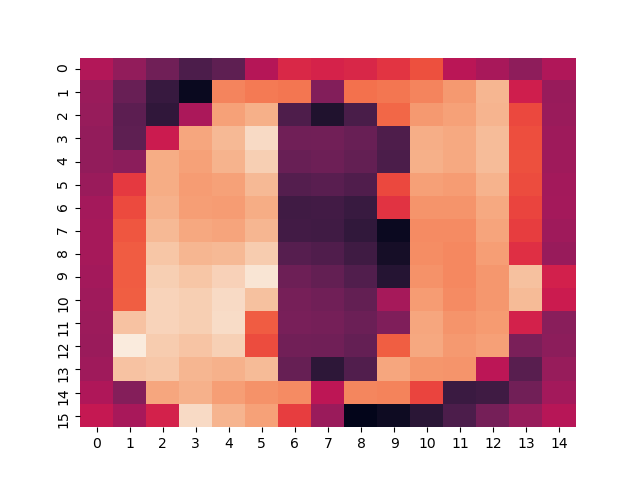
\includegraphics[scale=.12]{o0}
            \end{subfigure}
            \begin{subfigure}[c]{0.18\textwidth}
                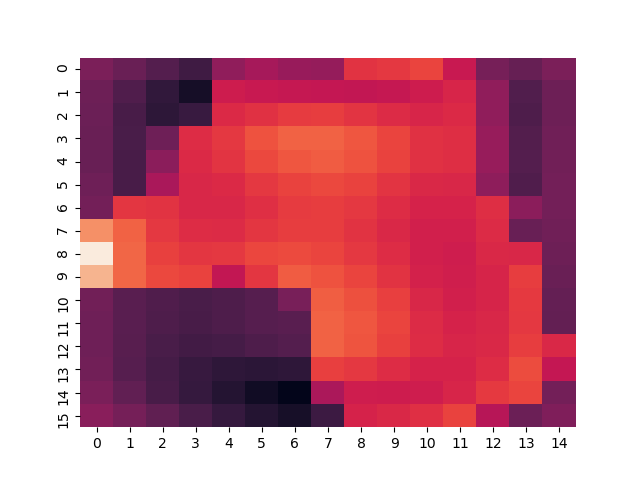
\includegraphics[scale=.12]{o1}
            \end{subfigure}
            \begin{subfigure}[c]{0.18\textwidth}
                \includegraphics[scale=.12]{o2}
            \end{subfigure}
            \begin{subfigure}[c]{0.18\textwidth}
                \includegraphics[scale=.12]{o3}
            \end{subfigure}
            \begin{subfigure}[c]{0.18\textwidth}
                \includegraphics[scale=.12]{o4}
            \end{subfigure}
            \\
            \begin{subfigure}[c]{0.18\textwidth}
                \includegraphics[scale=.12]{o5}
            \end{subfigure}
            \begin{subfigure}[c]{0.18\textwidth}
                \includegraphics[scale=.12]{o6}
            \end{subfigure}
            \begin{subfigure}[c]{0.18\textwidth}
                \includegraphics[scale=.12]{o7}
            \end{subfigure}
            \begin{subfigure}[c]{0.18\textwidth}
                \includegraphics[scale=.12]{o8}
            \end{subfigure}
            \begin{subfigure}[c]{0.18\textwidth}
                \includegraphics[scale=.12]{o9}
            \end{subfigure}
            \caption{Échantillon d'images originales}
        \end{figure}
    \end{frame}

    \begin{frame}{Reconstruction collaborative: images reconstruites}
        \begin{figure}[h]
            \centering
            \begin{subfigure}[c]{0.18\textwidth}
                \includegraphics[scale=.12]{0}
            \end{subfigure}
            \begin{subfigure}[c]{0.18\textwidth}
                \includegraphics[scale=.12]{1}
            \end{subfigure}
            \begin{subfigure}[c]{0.18\textwidth}
                \includegraphics[scale=.12]{2}
            \end{subfigure}
            \begin{subfigure}[c]{0.18\textwidth}
                \includegraphics[scale=.12]{3}
            \end{subfigure}
            \begin{subfigure}[c]{0.18\textwidth}
                \includegraphics[scale=.12]{4}
            \end{subfigure}
            \\
            \begin{subfigure}[c]{0.18\textwidth}
                \includegraphics[scale=.12]{5}
            \end{subfigure}
            \begin{subfigure}[c]{0.18\textwidth}
                \includegraphics[scale=.12]{6}
            \end{subfigure}
            \begin{subfigure}[c]{0.18\textwidth}
                \includegraphics[scale=.12]{7}
            \end{subfigure}
            \begin{subfigure}[c]{0.18\textwidth}
                \includegraphics[scale=.12]{8}
            \end{subfigure}
            \begin{subfigure}[c]{0.18\textwidth}
                \includegraphics[scale=.12]{9}
            \end{subfigure}
            \caption{Échantillon d'images reconstruites (~90\% des images 
            reconstruites)}
        \end{figure}
    \end{frame}

    \begin{frame}{Comparaison}
        \begin{figure}[h]
            \centering
            \begin{subfigure}[c]{0.3\textwidth}
                \includegraphics[scale=.20]{o6}
            \end{subfigure}
            \begin{subfigure}[c]{0.3\textwidth}
                \includegraphics[scale=.20]{6}
            \end{subfigure}
            \hfill
            \caption{Capture de l'information intrinsèque.}
        \end{figure}
    \end{frame}

    \begin{frame}{Reconstruction collaborative: images améliorables}
        \begin{figure}[h]
            \centering
            \begin{subfigure}[c]{0.18\textwidth}
                \includegraphics[scale=.12]{00}
            \end{subfigure}
            \begin{subfigure}[c]{0.18\textwidth}
                \includegraphics[scale=.12]{11}
            \end{subfigure}
            \begin{subfigure}[c]{0.18\textwidth}
                \includegraphics[scale=.12]{22}
            \end{subfigure}
            \begin{subfigure}[c]{0.18\textwidth}
                \includegraphics[scale=.12]{33}
            \end{subfigure}
            \begin{subfigure}[c]{0.18\textwidth}
                \includegraphics[scale=.12]{44}
            \end{subfigure}
            \\
            \begin{subfigure}[c]{0.18\textwidth}
                \includegraphics[scale=.12]{55}
            \end{subfigure}
            \begin{subfigure}[c]{0.18\textwidth}
                \includegraphics[scale=.12]{66}
            \end{subfigure}
            \begin{subfigure}[c]{0.18\textwidth}
                \includegraphics[scale=.12]{77}
            \end{subfigure}
            \begin{subfigure}[c]{0.18\textwidth}
                \includegraphics[scale=.12]{88}
            \end{subfigure}
            \begin{subfigure}[c]{0.18\textwidth}
                \includegraphics[scale=.12]{99}
            \end{subfigure}
            \caption{Échantillon d'images reconstruites (~10\% des images 
            reconstruites)}
        \end{figure}
    \end{frame}

    \begin{frame}{Reconstruction collaborative: un peu plus loin}
        \begin{itemize}
            \item Les données sont reconstruites pour \textbf{ensuite} être 
                utilisées
            \item Cas d'application: \textbf{la classification} (ici avec des 
                Random Forests)
            \item Est-ce que les individus reconstruits sont utilisables pour 
                des applications ultérieures ?\\~\\
            \item \textbf{Critère: différence en classification}: différence entre le 
                score utilisant les données originales et celui utilisant les 
                données reconstruites.
        \end{itemize}
    \end{frame}

    \begin{frame}{Reconstruction collaborative: un peu plus loin}
        \begin{figure}[!h]
            \centering
            \begin{subfigure}[c]{0.45\textwidth}
                \includegraphics[scale=.26]{cs_wdbc}
                \caption{WDBC}
            \end{subfigure}
            \begin{subfigure}[c]{0.45\textwidth}
                \includegraphics[scale=.26]{cs_mfeat}
                \caption{MFDD}
            \end{subfigure}\\
            \begin{subfigure}[c]{0.45\textwidth}
                \includegraphics[scale=.26]{cs_madelon}
                \caption{Madelon}
            \end{subfigure}
            \caption{Différences en classification par vue et par jeu de 
            données}
        \end{figure}
    \end{frame}

    \begin{frame}{Reconstruction collaborative: efficacité de la MWM}

        \begin{itemize}
            \item Nouveau jeu de données \textbf{artificiel}: Cube
            \item 1000 individus décrits par 
                3 descripteurs
            \item chaque vue est créée en \textbf{supprimant} une des dimensions
            \item \textbf{Objectif}: Tester la capacité de la méthode de 
                pondération par masque à \textbf{détecter quels descripteurs 
                sont pertinents}.
        \end{itemize}
        \begin{figure}[h]
            \centering
            \begin{subfigure}[h]{0.49\textwidth}
                \centering
                \includegraphics[width=0.9\textwidth]{data}
                \caption{Jeu de données Cube}
            \end{subfigure}
            \begin{subfigure}[h]{0.49\textwidth}
                \centering
                \includegraphics[width=0.9\textwidth]{projection0}
                \caption{Projection}
            \end{subfigure}
        \end{figure}
    \end{frame}

    \begin{frame}{Reconstruction collaborative: efficacité de la MWM}
        \begin{itemize}
            \item La méthode de pondération par masque \textbf{améliore les 
                résultats en reconstruction}.
            \item La sélection des features reconstruits \textbf{fonctionne 
                t-elle en pratique} ?
        \end{itemize}
        \begin{figure}[h]
            \centering
            \includegraphics[scale=.24]{process_mwm.png}
            \caption{Combinaison de deux individus partiellement corrects}
        \end{figure}
    \end{frame}

    \begin{frame}{Reconstruction collaborative: efficacité de la MWM}
        \begin{table}[h]
            \centering
            \begin{tabular}{ccc}
                \textbf{}                                       & 
                \parbox[c]{3cm}{\centering Moyenne} & \parbox[c]{3cm}{\centering 
                Écart type} \\ \midrule
                \textbf{Descripteur partagé}                         & 0.920    
                & 
                0.026                  \\ \midrule
                \multicolumn{1}{l}{\textbf{Descripteur non partagé}} & 0.143    
                & 
                0.034                  \\ \midrule
            \end{tabular}
            \caption{Moyenne et écart-type des paramètres des masques en 
            fonction du descripteur qu'elles pondèrent}
        \end{table}
        \begin{itemize}
            \item Les masques arrivent à \textbf{cibler les descripteurs 
                partagés} tout en \textbf{limitant l'utilisation des 
                descripteurs non partagés}.
            \item Le faible écart type indique une certaine \textbf{stabilité} 
                de la méthode
        \end{itemize}
    \end{frame}

    \begin{frame}{Reconstruction collaborative: résumé}
        Contributions
        \begin{itemize}
            \item Définition d'un nouveau \textbf{cas d'application du paradigme
                collaboratif}.
            \item Définition d'un système permettant de \textbf{reconstruire de manière
                collaborative} et basé sur des \textbf{réseaux de neurones}.
            \item Définition d'une méthode permettant de \textbf{combiner efficacement
                un ensemble de reconstructions}.\\~\\
        \end{itemize}
        Résultats
        \begin{itemize}
            \item Scores \textbf{améliorables} en reconstruction.
            \item Reconstruction \textbf{conserve une information intrinsèque}.
            \item \textbf{Sécurisation} des données
            \item Proof of concept, mais le système global doit être 
                \textbf{amélioré}.

        \end{itemize}
    \end{frame}

    \section{Contributions et Perspectives}
    \begin{frame}{Contributions}
        Dans cette thèse, nous avons proposé les trois contributions suivantes:
        \begin{itemize}
            \item Un algorithme de clustering collaboratif incrémental 
                permettant une adaptation des clusters aux éventuelles 
                évolutions de la distribution des données.
            \item Une méthode de pondération automatique des vues externes 
                permettant d'améliorer la qualité des collaborations lors d'un 
                clustering collaboratif.
            \item L'application du paradigme collaboratif au problème de la 
                reconstruction de données manquantes.
        \end{itemize}
    \end{frame}

    \begin{frame}{Apports de la thèse}
        Les apports de la thèse concernent les deux domaines suivants:
        \begin{itemize}
            \item Le clustering collaboratif incrémental
                \begin{itemize}
                    \item (article) ICONIP 2017
                    \item (article) EGC 2018
                \end{itemize}
            \item L'adaptation automatique de paramètres collaboratifs
                \begin{itemize}
                    \item (article) IJCNN 2018
                \end{itemize}
            \item La reconstruction collaborative
                \begin{itemize}
                    \item (journal, en cours de soumission) KAIS
                \end{itemize}
        \end{itemize}
    \end{frame}

    \begin{frame}{Perspectives}
        \begin{itemize}
            \item Analyse du comportement aux limites de la méthode de 
                clustering collaboratif incrémental.\\~\\
            \item Amélioration de chaque module utilisé pour le système de 
                reconstruction collaborative, en particulier les liens 
                permettant d'obtenir les reconstructions intermédiaires.\\~\\
            \item Étude théorique et approfondissement du paradigme de
                reconstruction collaborative: définition des conditions de
                transférabilité et de confidentialités des informations
                inter-vues, attestation de la qualité des individus
                reconstruits.
        \end{itemize}
    \end{frame}

    \begin{frame}
        \begin{center}
            Merci pour votre attention.\\
            Questions ?
        \end{center}
    \end{frame}

    %\begin{frame}{Bibliographie}
        %\bibliographystyle{abbrvnat}
        %\bibliography{./bib}
    %\end{frame}


    \appendix
    \begin{frame}{Descriptions des jeux de données}
        \begin{itemize}
            \item
                \textbf{WDBC}
                \begin{itemize}
                    \item 569
                    \item 3 $\times$ 10 descripteurs sur 1 type de cellule
                    \item description des caractéristiques physiques de chaque
                        cellule (rayon, texture, aire\ldots)
                \end{itemize}
            \item \textbf{Waveform}
                \begin{itemize}
                    \item 5000 individus
                    \item 40 attributs, 19 uniquement composés de bruits
                    \item les 21 attributs restants sont bruités et composés de
                        2 des 3 ``waves'' de base.
                \end{itemize}
            \item \textbf{Isolet}
                \begin{itemize}
                    \item 150 personnes ont prononcé chaque lettre de
                        l'alphabet deux fois.
                    \item les descripteurs sont des coefficients d'analyse
                        spectrale utilisée dans les études d'analyse de la
                        voix (l'ordre a été perdu).
                \end{itemize}
        \end{itemize}
    \end{frame}

    \begin{frame}{Descriptions des jeux de données}
        \begin{itemize}
            \item \textbf{Spambase}
                \begin{itemize}
                    \item 4601 mails (spam et non spam)
                    \item les descripteurs sont majoritairement (46/57) des
                        fréquences d'apparitions de mots dans les messages. Les
                        autres descripteurs sont soit des fréquences
                        d'apparition de caractères (6/51) soit des
                        caractéristiques propres aux séquences de lettres
                        écrites en capital.
                \end{itemize}
            \item \textbf{MFD}
                \begin{itemize}
                    \item 2000 chiffres manuscrits
                    \item chaque vue décrit l'ensemble de chiffres à l'aide de
                        coefficients utilisés en descriptions de l'image
                        (coefficients de Fourier, profile correlations,
                        coefficients de Karhunen-Love, moyennes de pixels,
                    moments de Zernike et des descripteurs morphologiques).
                \end{itemize}
            \item \textbf{Madelon}
                \begin{itemize}
                    \item 4400 individus artificiels (NIPS 2003)
                    \item 32 clusters placés aux somments d'un cube à 5 dimensions.
                    \item ajout de 480 descripteurs de bruit.
                \end{itemize}
        \end{itemize}
    \end{frame}

    \begin{frame}{Descriptions des jeux de données}
        \begin{itemize}
            \item \textbf{VHR Strasbourg}
                    \begin{itemize}
                        \item Segments d'images satellitse en très haute résolution 
                        \item 27 descripteurs décrivant les variations de couleur
                            sur chaque canal (rouge, vert, bleu et infra-rouge).
                    \end{itemize}
        \end{itemize}
    \end{frame}

    \begin{frame}{Mise à jour d'une SOM collaborative}
        Mise à jour des prototypes d'une carte SOM

        \begin{equation*}
            \forall w_n \in W, \quad w_n^{new} = w_n^{old} + \sum_{x_i} 
            K_{n,\chi(x_i)} \left( x_i - \chi(x_i) \right)
        \end{equation*}

        Définition des sous-critères locaux et collaboratifs

        \begin{equation*}
            Q_{local}^v = \alpha_v \sum_{x_i} \sum_{w_n \in W^v} 
            K_{n,\chi(x_n)}^v\|x_i - w_n \|_2
        \end{equation*}

        \begin{equation*}
            Q_{collab}^v = \sum_{v' \neq v}\beta_v^{v'} \sum_{x_i}\sum_{w_n \in 
            W^v} \big(K^v_{n,\chi(x_i)} - K^{v'}_{n,\chi(x_i)}\big)\|x_i - w_n 
        \|_2 \end{equation*}

        \begin{equation*}
            {w_n}^{new} = {w_n}^{old} - \epsilon \, \frac{\partial \left(  
            Q^v_{local} + Q^v_{collab} \right) }{\partial w_n}
        \end{equation*}
    \end{frame}

    \begin{frame}{Références}
        \begin{itemize}
            \item \textbf{(Deng2000)} Da Deng and Nikola Kasabov. Esom: An algorithm to
                evolve self-organizing maps from online data streams. In
                \textit{Neural Networks}, volume-6, page 3-8. IEEE, 2000.
            \item \textbf{(Ghassany2012)} Mohammad Ghassany, Nistor Grozavu, and Younès
                Bennani. Collaborative generative topographic mapping. In
                \textit{Internation Conference on Neural Information
                Processing}, pages 591-598. Springer, 2012.
            \item \textbf{(Grozavu2010)} Nistor Grozavu and Younès Bennani. Topological
                collaborative clutering. \textit{Australian Journal of
                Intelligent Information Processing Systems}, 12(2), 2010.
            \item \textbf{(Grozavu2011)} Nistor Grozavu, Mohamad Ghassany, and Younès
                Bennani. Learning confidence exchange in collaborative
                clustering. In \textit{Neural Networks (IJCNN), The 2011
                International Joint Conference on}, pages 872 879. IEEE, 2011.
        \end{itemize}
    \end{frame}

    \begin{frame}{Références}
        \begin{itemize}
            \item \textbf{(Kuhn1951)} Harold W. Kuhn and Albert W. Tucker. Nonlinear
                programming. In \textit{Proceeding of 2nd Berkeley Symposium},
                pages 481-492. 1951.
            \item \textbf{(Paplinski2012)} Andrew P.
                Paplinski. Incremental self-organizing map (isom) in
                categorization of visual objects. In \textit{ICONIP}, pages
                125-132. Springer, 2012.
            \item \textbf{(Pedrycz2002)} Witold Pedrycz.
                Collaborative fuzzy clustering. \textit{Pattern Recognition
                Letters}, 23(14):1675-1686, 2002.
            \item \textbf{(Pedrycz2004)} Witold
                Pedrycz. Fuzzy clustering with a knowledge-based guidance.
                \textit{Pattern Recognition Lettrs}, 25(4):469-480, 2004.
            \item \textbf{(Kohonen1982)} Teuvo Kohonen. Self-Organized Formation of 
                Topologically Correct Feature Maps. \textit{Biological 
                Cybernetics}. 43(1):59-69, 1982.
        \end{itemize}
    \end{frame}

    \begin{frame}{Complexité algorithme du clustering collaboratif}
        On ne tient pas compte du coût de calcul des méthodes implémentées par le clustering collaboratif.

        \begin{itemize}
            \item Complexité de \textbf{chaque algorithme local}
            \item Bande passante nécessaire au transfert des résultats 
                intermédiaires \textbf{proportionnelle au nombre d'individus} 
        \item Transferts répétés pour \textbf{chaque itération}
    \end{itemize}

        La reconstruction collaborative limite la quantité d'information transférées en ne les transférant qu'une seule fois.

        \begin{itemize}
            \item Apprentissage de $\mathbf{N}$ autoencodeur
            \item Par vue, apprentissage de $\mathbf{N-1}$ perceptron 
                multi-couches
            \item Par vue, apprentissage de $\mathbf{N-1}$ masques
        \end{itemize}
    \end{frame}

    \begin{frame}{Contexte générale}
        \begin{itemize}
            \item Thèse \textbf{exploratoire}
            \item Sujet initial plus orienté sur \textbf{l'analyse de données 
                appliquée au profilage de joueur}.\\~\\
            \item Difficultés liées à la \textbf{récupération des données}
            \item Difficultés liées à la \textbf{définition et à la portée du 
                sujet}
            \item Orientation du sujet vers le clustering collaboratif suite 
                \textbf{au premier comité de tiers parcours} sur conseil des 
                membres du comité.
        \end{itemize}
    \end{frame}
\end{document}
